\section{Procedimentos e resultados}

\par Para que esta pesquisa fosse levada a cabo, se fez necessária a implementação de algumas ações, as quais serão detalhadas.

\par O início da pesquisa deu-se através da escolha do tema, seguido pelo levantamento das tecnologias que seriam utilizadas. A princípio, foi definido um escopo contendo algumas tecnologias que haviam sido ministradas no ambiente acadêmico, diminuindo assim a curva de aprendizado. No entanto, foi preciso agregar alguns conhecimentos novos, despendendo um tempo maior para estudo. As tecnologias que acompanharam o desenvolvimento deste trabalho até a sua conclusão estão descritas no quadro teórico desta pesquisa.

\par Para garantir que as tecnologias selecionadas fossem as melhores para o desenvolvimento, foram realizados alguns testes, por meio de aplicações simples. Os testes foram focados na avaliação do comportamento do banco de dados aplicado ao contexto desta pesquisa, cujo objetivo foi desenvolver uma aplicação de busca por mão de obra baseando-se em uma rede de relacionamentos. Estes testes também foram realizados como fins didáticos, visando gerar a familiarização com as tecnologias utilizadas.

\par Para nortear este trabalho, usou-se uma metodologia de desenvolvimento, apresentada a seguir.

\subsection{Iconix}

\par O Iconix foi escolhido como a metodologia de desenvolvimento de \textit{software}, desempenhando um papel fundamental na organização. Sua abordagem proveu uma sequência de procedimentos, levando à construção de uma aplicação estável. Como relatado no quadro teórico, foram seguidas as quatro fases definidas pelo Iconix,

\par Na primeira fase, definida como análise de requisitos, foi realizado o levantamento das informações pertinentes ao desenvolvimento. Este levantamento foi realizado por meio da observação do comportamento das pessoas ao buscar por mão de obra temporária. A partir daí, foram levantadas as principais características, indispensáveis para a construção do \textit{software} e desenvolvido o modelo de domínio inicial, como demonstra a Figura~\ref{fig:modelo_dominio_inicial}.

\newpage
\begin{figure}[h!]
	\centerline{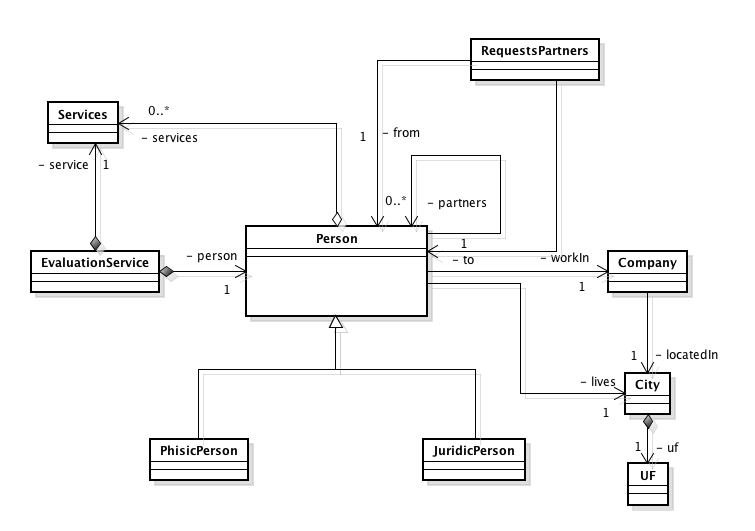
\includegraphics[scale=0.45]{./imagens/modelo-dominio-inicial.png}}
	\caption[Modelo de domínio inicial]
	{Modelo de domínio inicial. \textbf{Fonte:} Elaborado pelos autores.}
	\label{fig:modelo_dominio_inicial}
\end{figure}

\par Nesta fase, também foram definidas todas as ações cujo usuário poderia realizar no sistema, por meio dos casos de uso, conforme a Figura~\ref{fig:caso_uso_unificado}.

\newpage
\begin{figure}[h!]
	\centerline{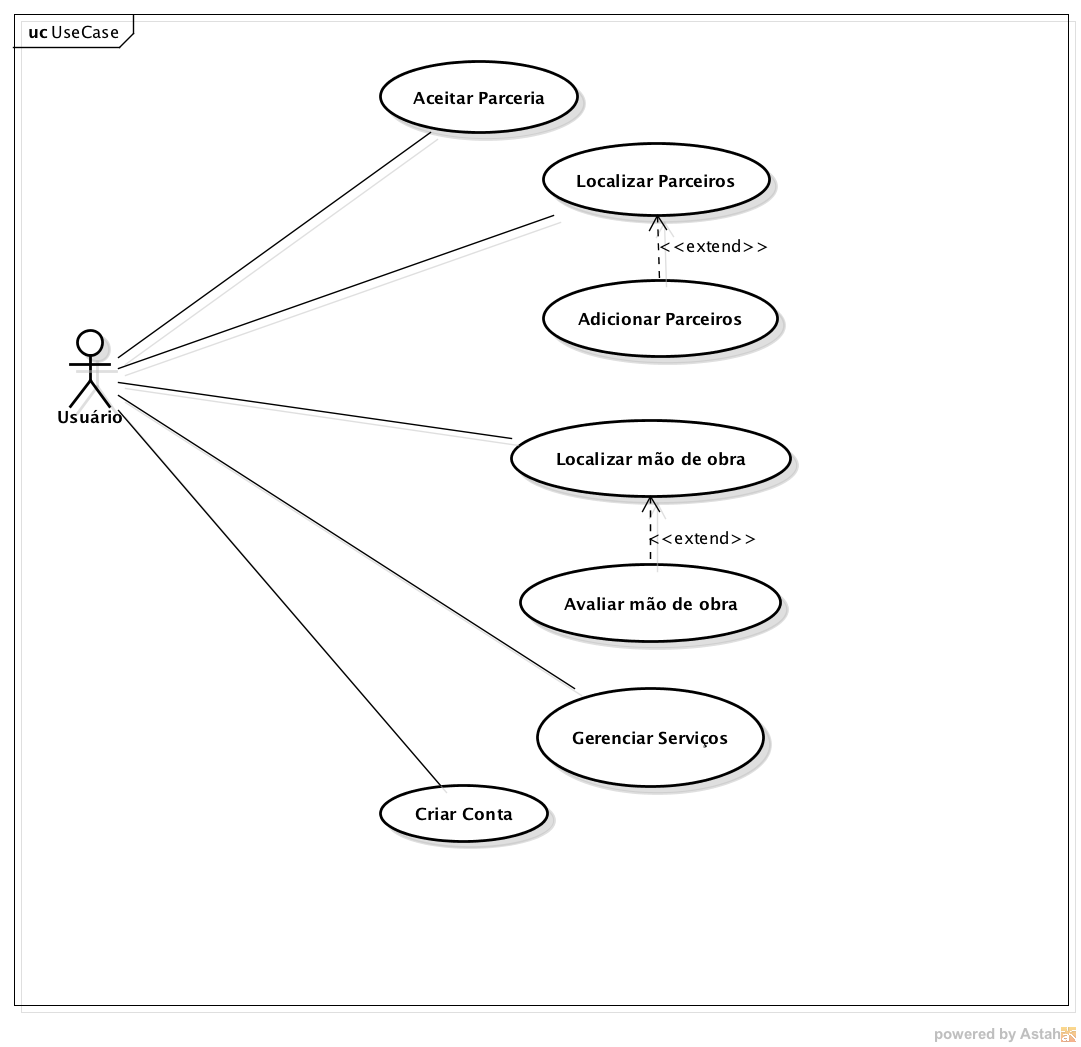
\includegraphics[scale=0.5]{./imagens/caso-de-uso-unificado.png}}
	\caption[Diagrama de caso de uso]
	{Diagrama de caso de uso. \textbf{Fonte:} Elaborado pelos autores.}
	\label{fig:caso_uso_unificado}
\end{figure}

% Removido após a pré-banca, pois, agora só haverá apenas um tipo de usuário (Ambos) e não mais provedor de serviço e contratante
%\newpage
%\begin{figure}[h!]
%	\centerline{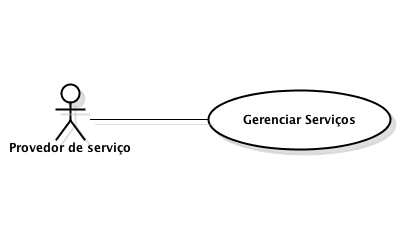
\includegraphics[scale=0.6]{./imagens/caso-de-uso-provedores-servico.png}}
%	\caption[Diagrama de caso de uso para provedores de serviços]
%	{Diagrama de caso de uso para provedores de serviços. \textbf{Fonte:} Elaborado pelos autores.}
%	\label{fig:caso_uso_provedor_servico_inicial}
%\end{figure}

%\begin{figure}[h!]
%	\centerline{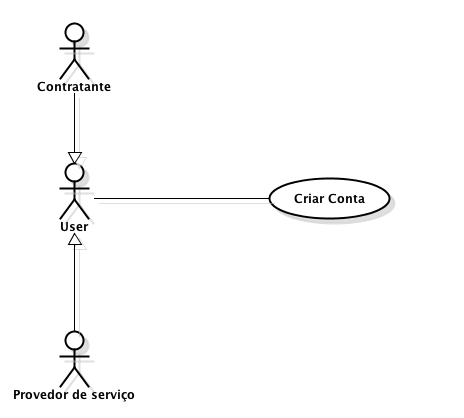
\includegraphics[scale=0.6]{./imagens/caso-de-uso-usuario.png}}
%	\caption[Diagrama de caso de uso para contratantes e provedores de serviços]
%	{Diagrama de caso de uso para contratantes e provedores de serviços. \textbf{Fonte:} Elaborado pelos autores.}
%	\label{fig:caso_uso_usuario_inicial}
%\end{figure}

\par Após definir os casos de uso, foram escritos os fluxos de eventos, para cada caso de uso. A seguir será apresentado o fluxo de eventos relacionado ao caso de uso ''Localizar parceiros'' por meio do Quadro~\ref{quad:fluxo_evento_localizar_parceiro}. Os demais fluxos de eventos são apresentados no Apêndice I em conjunto com os outros digramas deste trabalho.

% Conferir com o Márcio se os quadros serão removidos daqui e colocados nos apêndices depois só colar esta parte onde for inserida
%\newpage
%\begin{quadro}[h!]
%	\begin{fluxoDeEventos}
  \addTitle{Localizar Mão de obra}
  \addrow{Ator principal}{Contratante ou Ambos}
  \addrow{Ator secundário}{-}
  \addrow{Pré-condições}{O ator estar autenticado no sistema}
  \addrow{Pós-condições}{Provedores de serviço e suas respectivas mão de obras apresentadas ao ator.}
  
  \startBasicFlow{Ator} {Sistema}
  \addItemByColumnOne{O ator acessa a página para buscar o serviço por meio do menu “Busca” localizado no menu principal do sistema.}
  \addItemByColumnTwo{O sistema apresenta a página de busca de serviço e mão de obra.}
  
  \addItemByColumnOne{O ator informa qual a mão de obra que ele deseja pesquisar, por meio do campo “Buscar serviço”.}
  \addItemByColumnTwo{O sistema realiza uma busca pelo serviços que possuem o nome parecido com o nome do serviço informado pelo ator.ceiros que possuem maior probabilidade de se juntar a sua rede de parceiros.}
  
  \addItemByColumnOne{O ator seleciona o serviço a qual ele deseja que sejam pesquisados os provedores de serviço.}
  \addItemByColumnTwo{O sistema irá realizar a busca pela mão de obra solicitada pelo ator em sua base de dados, levando em consideração a rede de parceiros do ator, a empresa onde ele trabalha e a cidade onde o ator vive. Além é claro, da qualificação dos provedores de serviço. Após esta busca, o sistema apresentará uma página com a lista de prestadores de serviço que prestam tal mão de obra, ordenada pela credibilidade em sua rede de parceiros.}
  
  \addItemByColumnOne{O ator analisa a lista e seleciona a melhor opção a ele, clicando em sua imagem de perfil.}
  \addItemByColumnTwo{O sistema pesquisa todas as informações restantes do provedor de serviço, selecionado, pelo ator e apresenta uma página contendo todas as informações do provedor selecionado.}
   
  \startAlternativeFlow{Fluxo alternativo 1}
  \noAlternativeFlow{Não há fluxos alternativos}
\end{fluxoDeEventos}

%	\caption[Fluxo de eventos para o caso de uso ''localizar mão de obra'']
%	{Fluxo de eventos para o caso de uso ''localizar mão de obr''. \textbf{Fonte:} Elaborado pelos autores}
%	\label{quad:fluxo_evento_localizar_mao_de_obra}
%\end{quadro}

%\begin{quadro}[h!]
%	\begin{fluxoDeEventos}
  \addTitle{Avaliar Mão de obra}
  \addrow{Ator principal}{Contratante ou Ambos}
  \addrow{Ator secundário}{-}
  \addrow{Pré-condições}{O ator estar autenticado no sistema}
  \addrow{Pós-condições}{Mão de obra avaliada pelo ator}
  
  \startBasicFlow{Ator} {Sistema}
  \addItemByColumnOne{Após o item 6 do fluxo principal do fluxo de eventos “Localizar Mão de obra”. O ator clica no botão “Avaliar Serviço”.}
  \addItemByColumnTwo{O sistema apresenta o formulário de avaliação na mesma página para o ator.}
  
  \addItemByColumnOne{O ator preenche o formulário de avaliação da mão de obra e clica no botão “Salvar”.}
  \addItemByColumnTwo{O sistema registra a avaliação do cliente e apresenta uma mensagem de sucesso a ele.}
   
  \startAlternativeFlow{Fluxo alternativo 1}
  \noAlternativeFlow{Não há fluxos alternativos}
\end{fluxoDeEventos}

%	\caption[Fluxo de eventos para o caso de uso localizar mão de obra]
%	{Fluxo de eventos para o caso de uso localizar mão de obra. \textbf{Fonte:} Elaborado pelos autores}
%	\label{quad:fluxo_evento_avaliar_mao_de_obra}
%\end{quadro}

\newpage
\begin{quadro}[h!]
	\begin{fluxoDeEventos}
  \addTitle{Localizar Parceiros}
  \addrow{Ator principal}{Contratante ou Ambos}
  \addrow{Ator secundário}{-}
  \addrow{Pré-condições}{O ator estar autenticado no sistema}
  \addrow{Pós-condições}{Possíveis parceiro(s) apresentado(s) ao ator}
  
  

  \startBasicFlow{Ator} {Sistema}
  \addItemByColumnOne{O ator clica no menu “Rede de Parceiros” no menu principal localizado no menu principal do sistema.}
  \addItemByColumnTwo{O sistema apresenta a página contendo todos os parceiros ator e um campo para busca de novos parceiros.}
  
  \addItemByColumnOne{O ator informa o nome do parceiro que ele deseja encontrar no campo “Adicionar parceiros”.}
  \addItemByColumnTwo{O sistema pesquisa na sua base de dados os usuários que possuem aquele nome, e que por ventura, possuem algum tipo de ligação com os parceiros do ator, a fim de, tentar localizar os parceiros que possuem maior probabilidade de se juntar a sua rede de parceiros.}
  
  
  \startAlternativeFlow{Fluxo alternativo 1}
  \noAlternativeFlow{Não há fluxos alternativos}
\end{fluxoDeEventos}

	\caption[Fluxo de eventos para o caso de uso localizar parceiro]
	{Fluxo de eventos para o caso de uso localizar parceiro. \textbf{Fonte:} Elaborado pelos autores}
	\label{quad:fluxo_evento_localizar_parceiro}
\end{quadro}

%\newpage
%\begin{quadro}[h!]
%	\begin{fluxoDeEventos}
  \addTitle{Adicionar Parceiro}
  \addrow{Ator principal}{Contratante ou Ambos}
  \addrow{Ator secundário}{-}
  \addrow{Pré-condições}{O ator estar autenticado no sistema}
  \addrow{Pós-condições}{Parceiro(a) adicionado(a) a lista de parcerias do ator.}
  
  \startBasicFlow{Ator} {Sistema}
  \addItemByColumnOne{Após o item 4 do fluxo de eventos “Localizar Parceiros”. O ator clica na imagem de perfil do contratante a fim de, visualizar o perfil do possível novo parceiro.}
  \addItemByColumnTwo{O sistema realiza a busca das demais informações do contratante, cujo o ator selecionou para visualizar o perfil e apresenta a página de perfil dele ao ator.}
  
  \addItemByColumnOne{O ator visualiza o perfil do contratante e clique no botão “Adicionar Parceiro” para adicioná-lo  à sua lista de parceiros.}
  \addItemByColumnTwo{O sistema armazena esta requisição em sua base de dados, para aguardar a aprovação ou não do parceiro requisitado e apresenta uma mensagem de sucesso na requisição.}
 
  \startAlternativeFlow{Fluxo alternativo 1}
  \noAlternativeFlow{Não há fluxos alternativos}
\end{fluxoDeEventos}

%	\caption[Fluxo de eventos para o caso de uso adicionar parceiro]
%	{Fluxo de eventos para o caso de uso adicionar parceiro. \textbf{Fonte:} Elaborado pelos autores}
%	\label{quad:fluxo_evento_adicionar_parceiro}
%\end{quadro}

%\newpage
%\begin{quadro}[h!]
%	\begin{fluxoDeEventos}
  \addTitle{Aceitar Parceria}
  \addrow{Ator principal}{Contratante ou Ambos}
  \addrow{Ator secundário}{-}
  \addrow{Pré-condições}{O ator estar autenticado no sistema}
  \addrow{Pós-condições}{Novo(a) parceiro(a) adicionado(a) a lista de  parceiros do ator.}
  
  \startBasicFlow{Ator} {Sistema}
  \addItemByColumnOne{O ator acessa a página inicial do sistema personalizada a ele.}
  \addItemByColumnTwo{O sistema busca em sua base de dados todas as requisições de parcerias pendentes ao ator.}
  
  \addItemByColumnOne{Uma notificação push é apresentada ao ator no ícone “Novas Parcerias” do menu principal. Para visualizar a lista de requições pendentes, o ator deve passar o mouse sob este menu e um menu drop-down será apresentado ao ator contendo todas as requisições de parcerias.}
 
  \addEmptyColumn
  
  \addItemByColumnOne{Para responder a requisição o ator deve clicar no botão “confirmar” ou “cancelar” de cada uma das requisições da lista.}
  
  \addItemByColumnTwo{Ao clicar no botão “confirmar” o sistema confirma a parceria entre ambos os contratantes e apresenta uma mensagem de sucesso ao ator.}
  
  \startAlternativeFlow{Fluxo alternativo 1}
  \addItemByColumnOne{No item 4 do fluxo principal o ator clica no botão “cancelar” da requisição de parceria.}
  \addItemByColumnTwo{O sistema remove a requisição de parceria da sua base de dados, impedindo assim que a mesma requisição volte a ser apresentada ao ator.}
\end{fluxoDeEventos}

%	\caption[Fluxo de eventos para o caso de uso aceitar parceria]
%	{Fluxo de eventos para o caso de uso aceitar parceria. \textbf{Fonte:} Elaborado pelos autores}
%	\label{quad:fluxo_evento_aceitar_parceria}
%\end{quadro}

%\newpage
%\begin{quadro}[h!]
%	\begin{fluxoDeEventos}
  \addTitle{Gerenciar Serviços}
  \addrow{Ator principal}{Provedor de serviço}
  \addrow{Ator secundário}{-}
  \addrow{Pré-condições}{O ator estar autenticado no sistema}
  \addrow{Pós-condições}{Serviço atribuído ao ator.}
  
  \startBasicFlow{Ator} {Sistema}
  \addItemByColumnOne{O ator clica no menu “Serviço” apresentado na barra de menu principal do sistema.}
  \addItemByColumnTwo{O sistema apresenta a página contendo a lista de serviços prestados por ele, além do formulário para atrelar um novo serviço a ele.}
  
  \addItemByColumnOne{O ator começa a inserir o nome do serviço que deseja localizar.}
  \addItemByColumnTwo{O sistema realiza uma busca a fim de apresentar todas as opções possíveis de serviços anteriormente cadastradas no banco de dados , segundo o nome informado pelo ator.}
  
  \addItemByColumnOne{O ator seleciona o serviço que deseja atrelar a si mesmo por meio da lista de serviços apresentados e clica no botão “Adicionar”.}
  
  \addItemByColumnTwo{O sistema atrela o serviço ao ator com sucesso e apresenta uma mensagem de sucesso a ele.}
  
  \addItemByColumnOne{O ator lê a mensagem de sucesso.}
  \addEmptyColumn
  
  \startAlternativeFlow{Fluxo alternativo 1}
  \addItemByColumnTwo{No item 4 do fluxo principal, o sistema não localiza nenhum serviço em sua base de dados com o nome informado pelo ator e, portanto não apresenta nenhuma opção para seleção.}
  
  \addItemByColumnOne{O ator conclui o nome do serviço, caso seja necessário e clica no botão “Adicionar”.}
  \addItemByColumnTwo{O sistema verifica que o serviço não está registrado em sua base de dados, portanto, o cria e atrela ele ao ator. Após isto, apresenta uma mensagem de sucesso ao ator.}
  
  \addItemByColumnOne{O ator lê a mensagem de sucesso.}
  \addEmptyColumn
  
  
  \startAlternativeFlow{Fluxo alternativo 2}
  \addItemByColumnTwo{No item 6 do fluxo principal, o sistema realiza uma validação, a fim de evitar que o usuário atribua o mesmo serviço a si mesmo mais de uma vez.  Após isto, uma mensagem informando ao usuário sobre a falha é apresentada.}
  
  \addItemByColumnOne{O ator lê a mensagem de erro.}
  \addEmptyColumn
  
\end{fluxoDeEventos}

%	\caption[Fluxo de eventos para o caso de uso gerenciar serviços]
%	{Fluxo de eventos para o caso de uso gerenciar serviços. \textbf{Fonte:} Elaborado pelos autores}
%	\label{quad:fluxo_evento_gerenciar_servicos}
%\end{quadro}

%\newpage
%\begin{quadro}[h!]
%	\begin{fluxoDeEventos}
  \addTitle{Criar Conta}
  \addrow{Ator principal}{Usuário}
  \addrow{Ator secundário}{-}
  \addrow{Pré-condições}{}
  \addrow{Pós-condições}{Conta criada com sucesso}
  
  

  \startBasicFlow{Ator} {Sistema}
  \addItemByColumnOne{O ator acessa a página inicial do sistema.}
  \addItemByColumnTwo{O sistema apresenta a página de boas vindas ao usuário.}
  
  \addItemByColumnOne{O ator clica no menu “Criar conta” na barra de menu superior.}
  \addItemByColumnTwo{O sistema apresenta a tela para criar a nova conta.}
  
  \addItemByColumnOne{O ator preenche alguns campos relacionados aos seus dados pessoais e clica no botão “Próximo”.}
  \addItemByColumnTwo{O sistema armazena a nova conta e redireciona o ator para a página contendo o formulário correspondente ao segundo passo para concluir a criação de conta.}
  
  \addItemByColumnOne{O ator preenche alguns campos relacionados aos seus dados profissionais e clica no botão “Próximo”.}
  \addItemByColumnTwo{O sistema atualiza os dados da conta recém-criada e redireciona o ator para a página relacionada ao terceiro e último passo para criação da conta.}
  
  \addItemByColumnOne{O ator insere a sua imagem de perfil e clica no botão “Salvar”.}
  \addItemByColumnTwo{O sistema atualiza a conta recém-criada e redireciona o ator para a sua página inicial.}
  
  
  \startAlternativeFlow{Fluxo alternativo 1}
  \addItemByColumnTwo{No item 6 do fluxo principal, o sistema verifica que já existe um usuário com o mesmo e-mail.}
  
  \addItemByColumnTwo{O sistema apresenta uma mensagem de erro informando a situação ao ator.}
  
  \addItemByColumnOne{O ator lê a mensagem de erro.}
  \addItemByColumnTwo{O sistema mantém o estado atual da página, aguardando pela inserção de um e-mail válido.}
\end{fluxoDeEventos}

%	\caption[Fluxo de eventos para o caso de uso criar conta]
%	{Fluxo de eventos para o caso de uso criar conta. \textbf{Fonte:} Elaborado pelos autores}
%	\label{quad:fluxo_evento_criar_conta}
%\end{quadro}


\par Na segunda fase, análise e projeto preliminar, houve um refinamento dos requisitos levantados na fase anterior, aperfeiçoando as ações do usuário, por meio dos diagramas de casos de uso ou fluxos de eventos. Posterior a esta definição, foram desenvolvidos os diagramas de robustez, como demonstra a Figura~\ref{fig:diagrama_robustez_localizar_mao_de_obra}.

\newpage
\begin{figure}[h!]
	\centerline{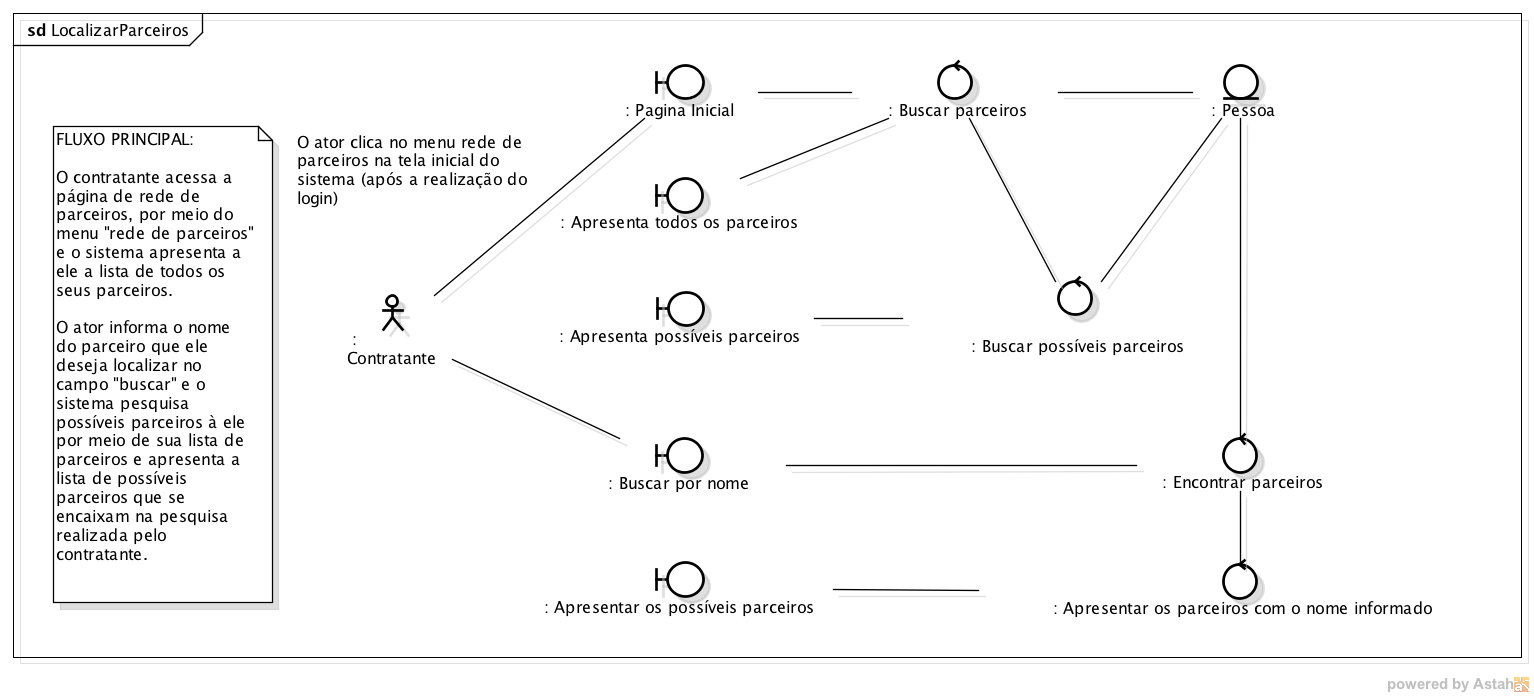
\includegraphics[scale=0.35]{./imagens/apendices/diagrama-robustez-localizar-parceiros.png}}
	\caption[Diagrama de robustez do caso de uso ''Localizar parceiros'']
	{Diagrama de robustez do caso de uso ''Localizar parceiros''. \textbf{Fonte:} Elaborado pelos autores.}
	\label{fig:diagrama_robustez_localizar_mao_de_obra}
\end{figure}

Em paralelo, foi atualizado o modelo de domínio, acrescentando os novos atributos identificados na segunda fase, conforme a Figura~\ref{fig:modelo_dominio_atualizado}.

\begin{figure}[h!]
	\centerline{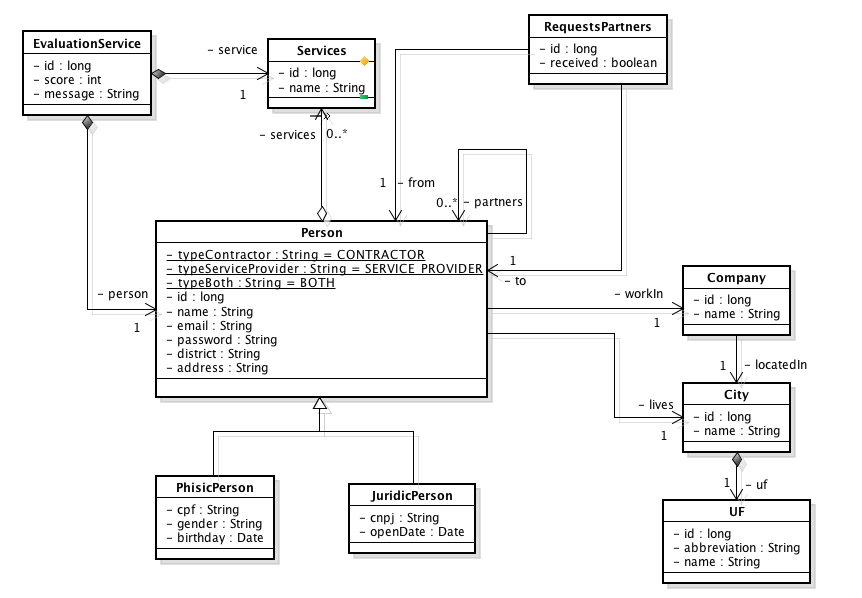
\includegraphics[scale=0.5]{./imagens/modelo-dominio-com-atributos.png}}
	\caption[Modelo de domínio atualizado]
	{Modelo de domínio atualizado. \textbf{Fonte:} Elaborado pelos autores.}
	\label{fig:modelo_dominio_atualizado}
\end{figure}

Com o modelo de domínio atualizado, foi feita a modelagem do banco de dados da aplicação, como apresenta a Figura~\ref{fig:modelo_dados_aplicacao}.

\begin{figure}[h!]
	\centerline{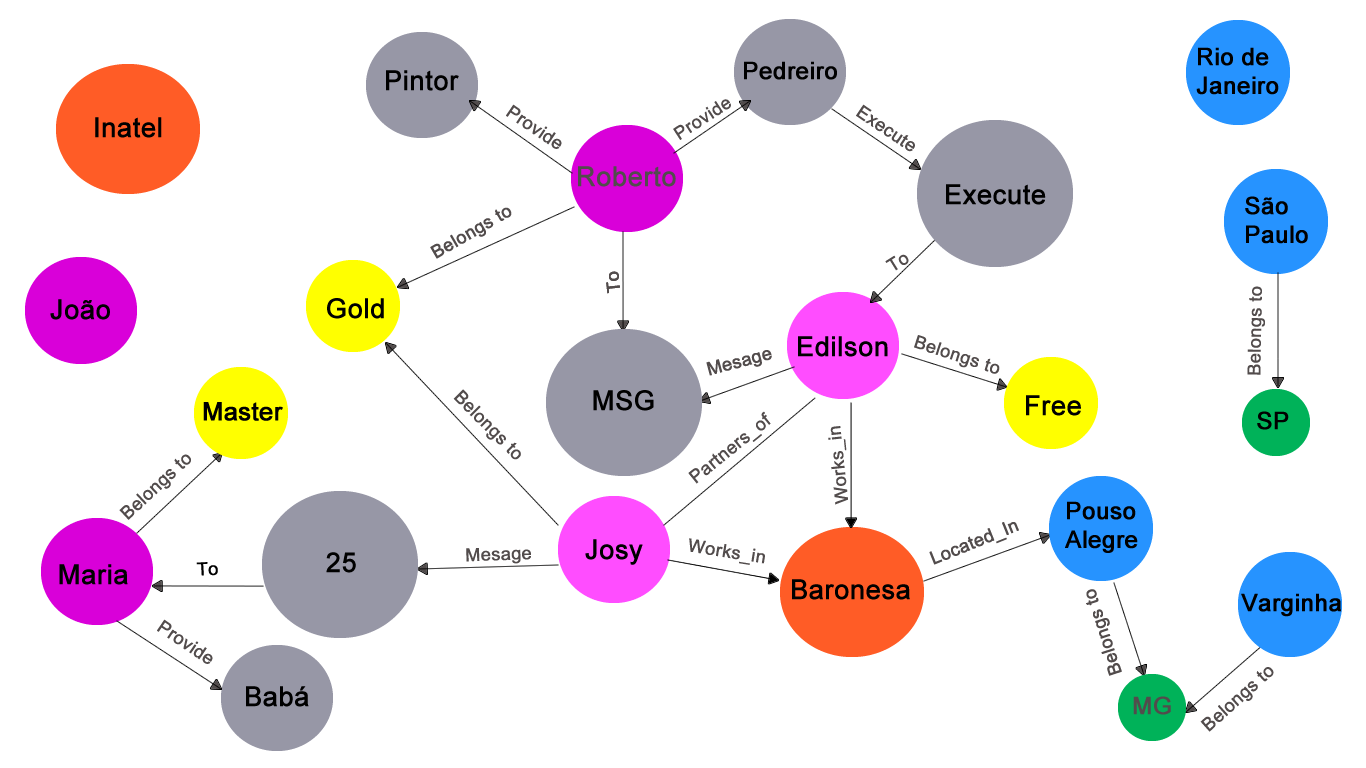
\includegraphics[scale=0.4]{./imagens/structure-all-nodes.png}}
	\caption[Modelo de dados da aplicação]
	{Modelo de dados da aplicação. \textbf{Fonte:} Elaborado pelos autores.}
	\label{fig:modelo_dados_aplicacao}
\end{figure} 

\par Na terceira fase, definida como projeto detalhado, foram criados os diagramas de sequência, tendo como base os casos de uso modelados na fase anterior. Esta fase tem como objetivo detalhar todo o funcionamento do \textit{software}, visando definir a melhor maneira de realizar sua implementação. A Figura~\ref{fig:diagrama_sequencia_localizar_parceiros} apresenta o diagrama de sequência do caso de uso ''Localizar parceiros''.

\newpage
\begin{figure}[h!]
	\centerline{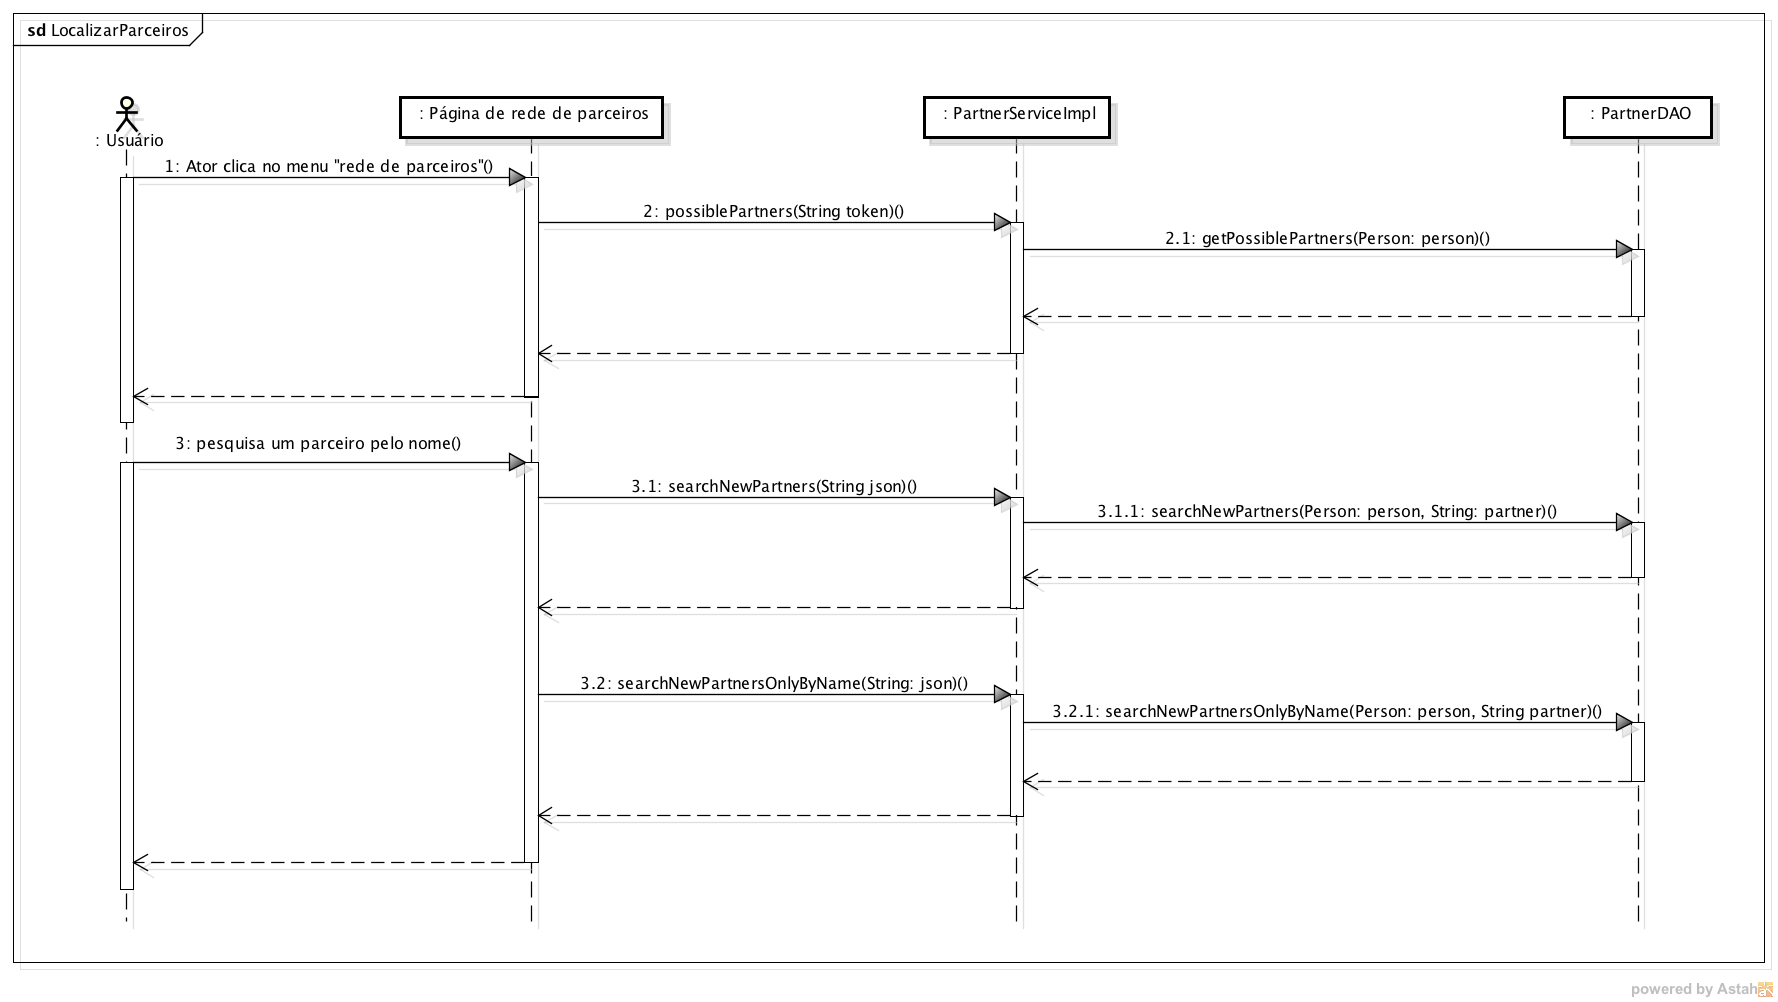
\includegraphics[angle=90,scale=0.4]{./imagens/diagrama-sequencia-localizar-novos-parceiros.png}}
	\caption[Diagrama de sequência do caso de uso ''Localizar parceiros'']
	{Diagrama de sequência do caso de uso ''Localizar parceiros''. \textbf{Fonte:} Elaborado pelos autores.}
	\label{fig:diagrama_sequencia_localizar_parceiros}
\end{figure}

\par Ainda na fase de projeto detalhado, após a modelagem dos diagramas de sequência, as operações encontradas nestes diagramas foram adicionadas ao modelo de domínio, em conjunto com as novas classes identificadas, gerando assim, o digrama de classes como mostra a Figura~\ref{fig:diagrama_classe}.

\begin{figure}[h!]
	\centerline{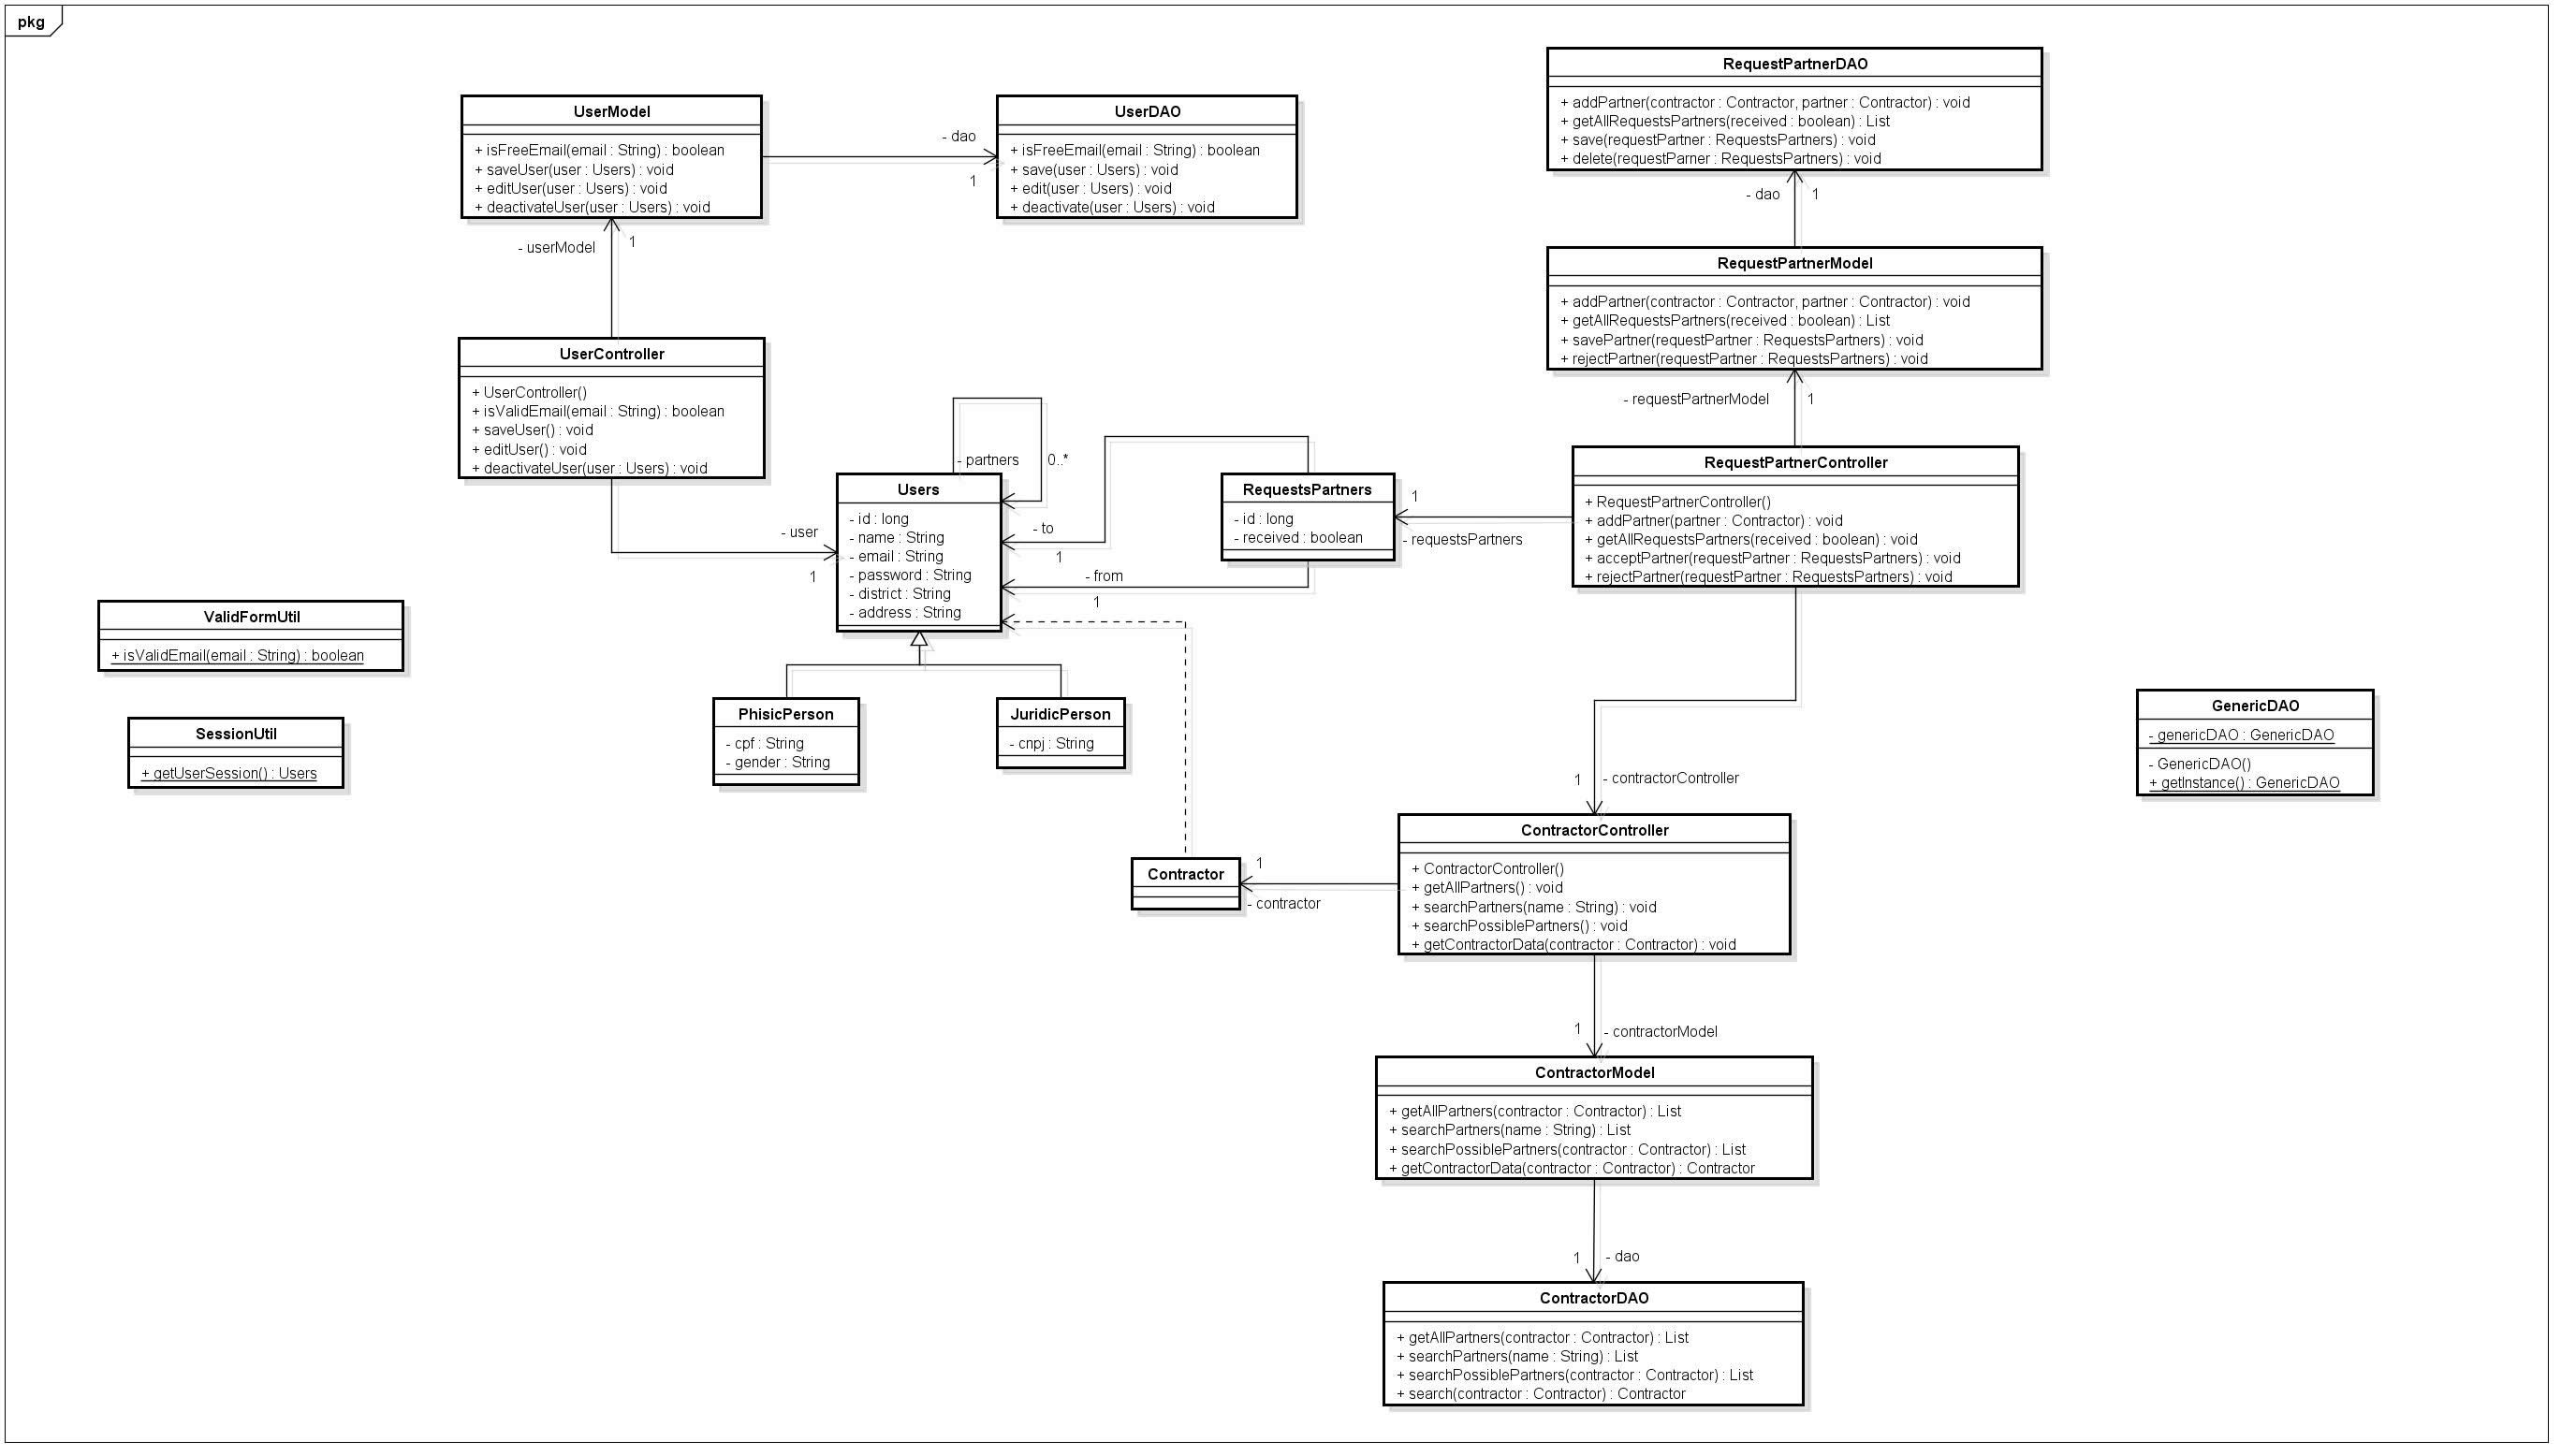
\includegraphics[angle=90,height=0.7\textheight,width=0.7\textwidth]{./imagens/classe.jpg}}
	\caption[Diagrama de classes]
	{Diagrama de classes \textbf{Fonte:} Elaborado pelos autores.}
	\label{fig:diagrama_classe}
\end{figure}

\newpage
\par Na quarta e última fase do ICONIX, denominada implementação, iniciou-se a preparação do ambiente, incluindo a instalação dos \textit{softwares} necessários para o desenvolvimento prático da aplicação. Essa preparação é abordada a seguir.


\subsection{Preparação do ambiente}

\par Visto que o trabalho seria desenvolvido em equipe, foi necessário estabelecer uma ferramenta de controle de versão. Esta ferramente permitiu o gerenciamento de diferentes versões de arquivos, mantendo um histórico com as modificações que foram realizadas no decorrer do processo de desenvolvimento. Este histórico permite o retorno de alguma revisão, caso haja necessidade. A ferramenta escolhida para realizar esse controle foi o GitHub, que já havia sido utilizado em alguns trabalhos do contexto acadêmico, evitando o desprendimento de tempo para estudo de uma nova ferramenta de apoio. O GitHub é uma ferramenta bem difundida e permite que os seus usuários colaborem com os projetos que estão armazenados em seus repositórios\footnotemark[31]. A Figura~\ref{fig:github_inicio} demonstra a tela de serviços provida pelo GitHub.

\footnotetext[31]{Repositório: local cujo desenvolvedor utiliza para armazenar os documentos relacionados ao \textit{software}.}

\begin{figure}[h!]
	\centerline{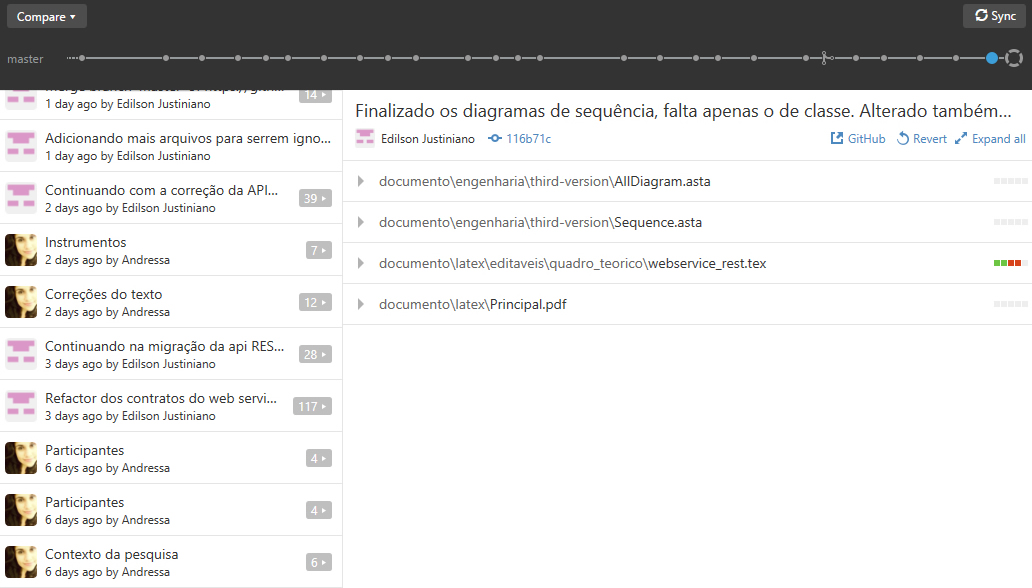
\includegraphics[scale=0.3]{./imagens/github.jpg}}
	\caption[Tela de serviços do GitHub ]
	{Tela de serviços do GitHub \textbf{Fonte:} Elaborado pelos autores.}
	\label{fig:github_inicio}
\end{figure}

\par Os passos de instalação detalhados do GitHub são descritos  no Apêndice III deste trabalho.

\par Como mencionado no quadro teórico, neste trabalho foi utilizada a linguagem Java, sendo assim necessária a utilização de uma \textit{Integrated Development Environment} - IDE\footnotemark[32] - de apoio. A IDE escolhida foi o Eclipse, pois se trata de uma ferramenta \textit{open source}, muito utilizada no mercado e que permite a escrita de um código mais legível, facilitando tarefas como \textit{debug} e configurações do trabalho.

\footnotetext[32]{IDE: \textit{Integrated Development Environment} - Aplicação contendo uma série de ferramentas para auxiliar no desenvolvimento de \textit{software}.}

\par O Eclipse possui várias ferramentas, dentre elas, pode-se citar o editor de texto, usado não somente para a escrita de códigos em Java, e também a perspectiva de configuração para servidores \textit{web}, utilizada neste trabalho, conforme apresenta a Figura~\ref{fig:ide_eclipse}. Por meio desta perspectiva, foi configurada a aplicação \textit{container} Tomcat na versão 7.

\begin{figure}[h!]
	\centerline{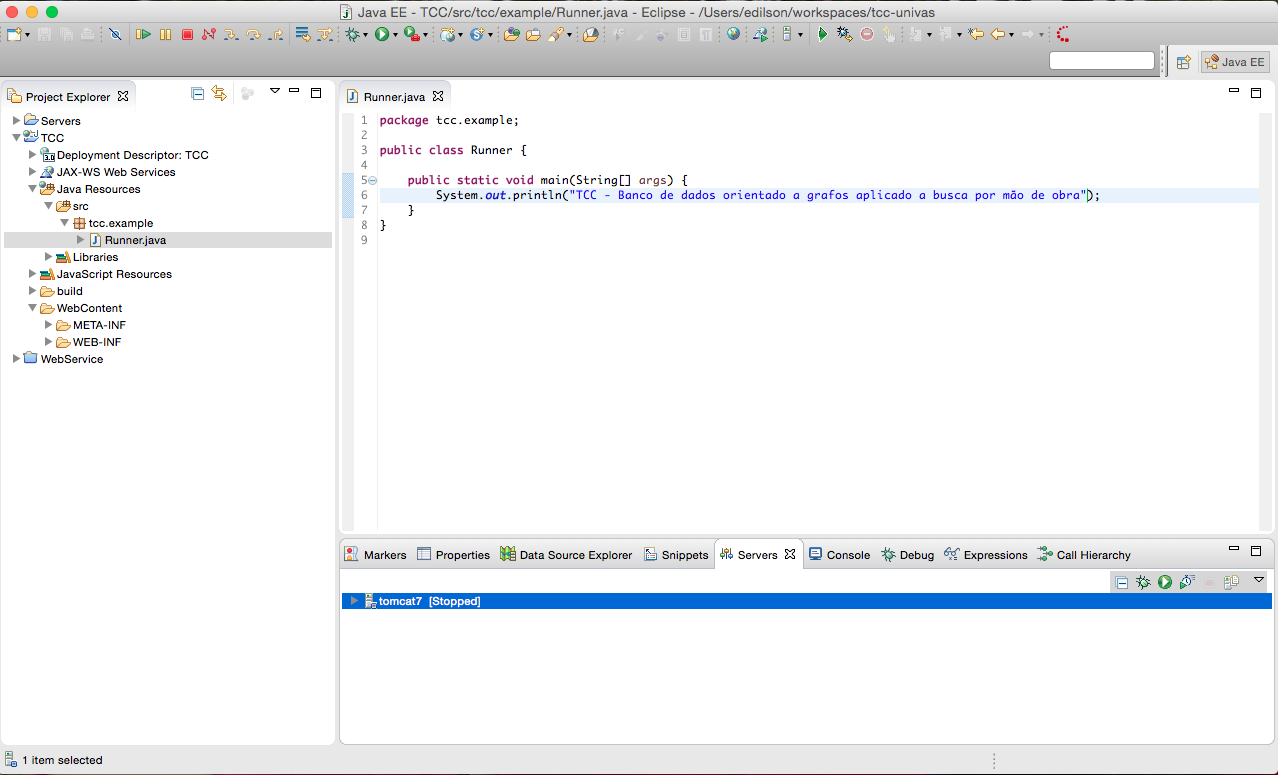
\includegraphics[scale=0.3]{./imagens/eclipse-editor-texto.png}}
	\caption[Ferramentas da IDE Eclipse]
	{Ferramentas da IDE Eclipse \textbf{Fonte:} Elaborado pelos autores.}
	\label{fig:ide_eclipse}
\end{figure}

\par O Tomcat desempenhou um papel fundamental na execução desta aplicação, pois serviu como hospedeiro para a aplicação Java desenvolvida neste trabalho. 

\par Os passos de instalação e configuração do Eclipse e do Tomcat são descritos no Apêndice IV deste trabalho.

\par Para a escrita do código relacionado ao HTML, CSS e Javascript, foi utilizado o mesmo editor de texto citado anteriormente.

\par O trabalho fez uso de um banco de dados orientado a grafos, o Neo4j. A escolha desse banco se deu pela sua simplicidade de instalação, configuração, facilidade de integração com a API \textit{Cypher} e por disponibilizar uma API REST para acesso aos seus dados, conforme descrito no quadro teórico deste trabalho. O Neo4j faz parte do enquadramento de softwares livres, seguindo o conceito \textit{open source}, o que permite ao desenvolvedor utilizá-lo da forma que melhor lhe convier. 

\par Os passos para a instalação do banco de dados Neo4j são detalhados no Apêndice V deste trabalho.

\par Posterior à configuração do ambiente, iniciou-se o desenvolvimento propriamente dito, apresentado a seguir.


\subsection{Desenvolvimento}

\par A princípio, utilizou-se as tecnologias Neo4j, sendo executado de forma \textit{embedded}, Primefaces e JSF. Porém não estava fluindo como o esperado. Outro problema encontrado ao utilizar tais tecnologias foi que tanto a parte cliente (\textit{front end}) quanto a parte servidor (\textit{back end}) se encontravam totalmente acoplados em uma aplicação Java \textit{web}. Por estes motivos decidiu-se mudar algumas das tecnologias utilizadas.

\par Posterior a esse incidente, passou-se a utilizar então as linguagens HTML 5, CSS 3, Javascript e o \textit{framework} Angular JS para auxiliar no desenvolvimento do \textit{front end}, ao invés de Primefaces e JSF. Para acesso ao banco de dados, lançou-se mão da forma \textit{embedded} e passou-se a utilizar a API REST disponibilizada pelo próprio banco. Tais decisões nos permitiram desacoplar o sistema e manter o \textit{front end} e o \textit{back end} independentes, evitando, assim, que o mesmo problema voltasse a ocorrer.

\par Como a forma de conexão ao banco de dados foi alterada, houve a necessidade de reescrever a classe responsável por realizar esta conexão, conforme apresenta o Código~\ref{list:codigo_comunicacao_banco}.

\begin{lstlisting} [style=custom_Java,caption={[Código de comunicação com o banco de dados]{Código de comunicação com o banco de dados. \textbf{Fonte:} Elaborado pelos autores.}}, label=list:codigo_comunicacao_banco] 	
public class FactoryDAO {

	private static final String DATABASE_ENDPOINT =
								 "http://localhost:7474/db/data";
	private static final String DATABASE_USERNAME = "neo4j";
	private static final String DATABASE_PASSWORD = "admin";
	private static final String cypherUrl = 
								 DATABASE_ENDPOINT + "/cypher";
	
	private static WebResource instance;
	
	private FactoryDAO() {
	}
	
	public static WebResource GetInstance() {
		WebResource resource = null;
		if (instance == null) {
			Client c = Client.create();
			c.addFilter(new HTTPBasicAuthFilter(DATABASE_USERNAME,
												DATABASE_PASSWORD));
			resource = c.resource(cypherUrl);
		}
		return resource;
	}
}
\end{lstlisting}

% Trocado de imagem para listagem
%\begin{figure}[h!]
%	\centerline{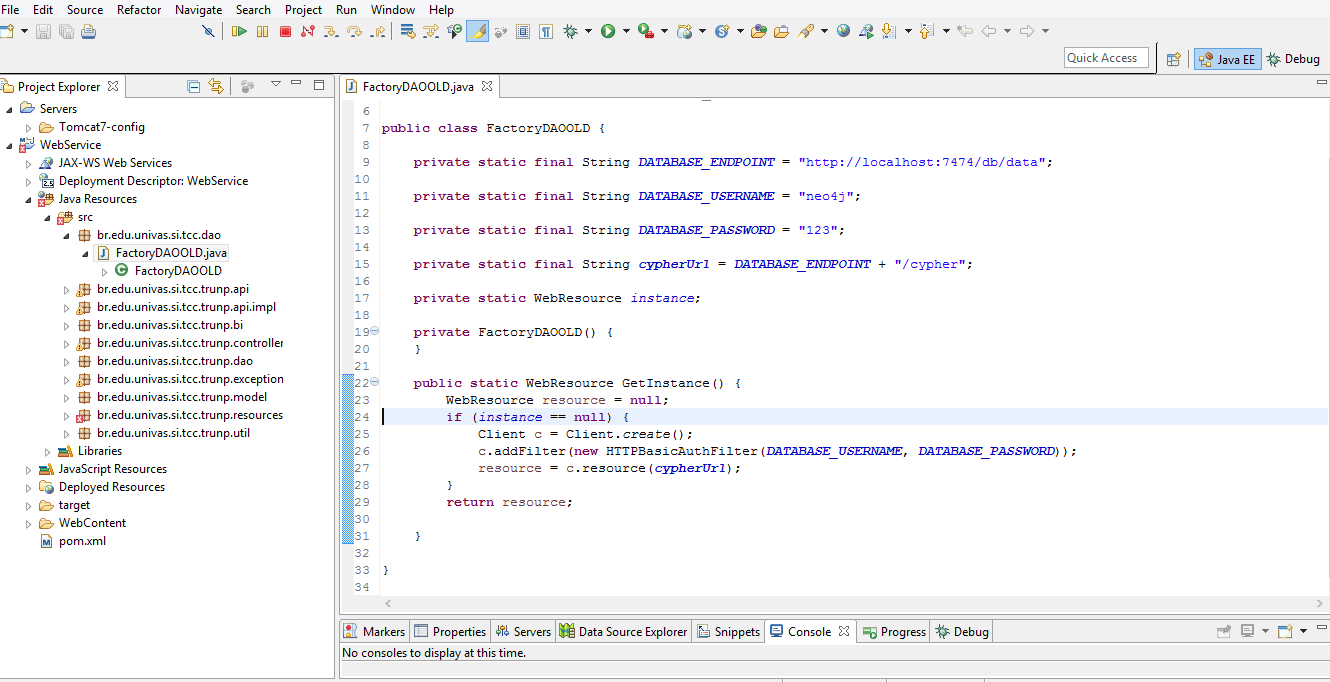
\includegraphics[scale=0.3]{./imagens/conexao-banco.jpg}}
%	\caption[Código de comunicação com o banco]
%	{Código de comunicação com o banco \textbf{Fonte:} Elaborado pelos autores.}
%	\label{fig:codigo_comunicacao_banco}
%\end{figure}

\par Após realizar a mudança de tecnologias, foram executados alguns procedimentos para compreender o funcionamento do \textit{web service} REST e em paralelo, foi feito o levantamento dos materiais de referência do \textit{framework} Angular JS. Foi preciso realizar testes para validar a conexão com o banco de dados Neo4j via API REST, fornecida por ele, além de realizados testes funcionais para envio de requisições e recebimento de respostas do \textit{web service} REST, utilizando o Angular JS. Para validar a conexão ao banco de dados via API REST foi necessário desenvolver algumas consultas em \textit{cypher}, como apresenta o Código~\ref{list:consulta_usando_api_cypher}.

\begin{lstlisting} [style=custom_Java,caption={[Exemplo de consulta usando a API \textit{cypher}]{Exemplo de consulta usando a API \textit{cypher}. \textbf{Fonte:} Elaborado pelos autores.}}, label=list:consulta_usando_api_cypher] 	

public class PersonDAO {
...

	/**
	* Used to get all data of person to show the profile data
	* 
	* @param partnerEmail
	* @return
	* @throws JSONException 
	*/
	public JSONArray getPersonData(String partnerEmail) throws JSONException {
		
		WebResource resource = FactoryDAO.GetInstance();
		
		String query = null;
		query = "{\"query\":\" MATCH (partner:Person {email: '"
			+ partnerEmail + "'}), (city:City), "
			+ "(company:Company), "
			+ "(partner)-[:LIVES_IN]->(city), "
			+ "(partner)-[:WORKS_IN]->(company) "
			+ "RETURN DISTINCT({name: partner.name, "
			+ "email: partner.email, photo: partner.photo, " 
			+ "city: city.name, company: company.name, " 
			+ "cpf: partner.cpf, cnpj: partner.cnpj, " 
			+ "typeOfPerson: partner.typeOfPerson, " 
			+ "gender: partner.gender}) as partner; \"}";
		ClientResponse responseCreate = resource
									.accept(MediaType.APPLICATION_JSON)
									.type(MediaType.APPLICATION_JSON).entity(query)
									.post(ClientResponse.class);
		String resp = responseCreate.getEntity(String.class);
		
		JSONObject json = new JSONObject(resp);
		JSONArray objData = json.getJSONArray("data");
		List<JSONObject> parser = JSONUtil
												.parseJSONArrayToListJSON(objData);
		JSONArray arr = new JSONArray(parser);
		
		return arr;
	}
...
}
\end{lstlisting}

% Trocado de imagem para listagem
%\begin{figure}[h!]
%	\centerline{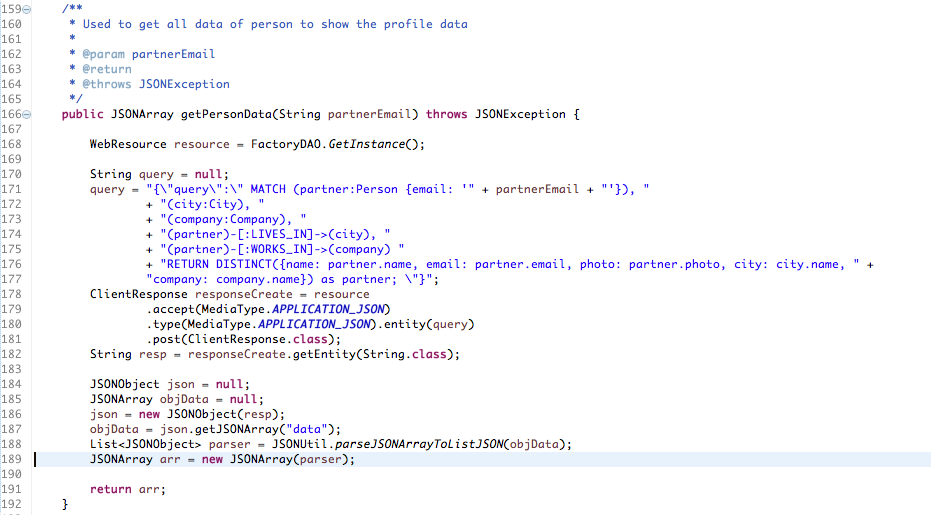
\includegraphics[scale=0.45]{./imagens/query-cypher.png}}
%	\caption[Exemplo de consulta usando a API \textit{cypher}]
%	{Exemplo de consulta usando a API \textit{cypher}. \textbf{Fonte:} Elaborado pelos autores.}
%	\label{fig:consulta_usando_api_cypher}
%\end{figure}

Nesse trecho de código entre as linhas 17 e 27 é apresentada uma consulta escrita usando a API \textit{Cypher}, ela tem por finalidade recuperar os dados de um determinado usuário. Como já mencionado no quadro teórico deste trabalho, o \textit{Cypher} utiliza algumas cláusulas, dentre elas é possível mencionar a \texttt{MATCH} e \texttt{RETURN} cuja utilização delas é apresentada nessa consulta. Na cláusula \texttt{MATCH} são definidos os padrões para realizar a busca, nesse caso, uma pessoa que viva em qualquer cidade, trabalhe em uma empresa qualquer e que possua o \textit{e-mail} igual ao recebido como parâmetro pelo método \texttt{getPersonData}. Já a clásula \texttt{RETURN}, são definidos os dados desejados pela consulta, nesse caso, são eles: o nome do usuário, o \textit{e-mail}, a foto, a cidade onde vive, a empresa onde trabalha, o CPF (em caso de pessoas físicas), o CNPJ (para pessoas jurídicas), o tipo da conta (pessoa jurídica ou física), e o sexo do usuário (usado para pessoas físicas). Mas como é possível notar, foi necessário gerar um objeto JSON manualmente contendo os dados desejados como pode ser visualizado a partir da linha 22 até a linha 27, pois, por padrão o Neo4j não retorna os resultados no formato JSON comum, como demonstra o Código~\ref{list:exemplo_json_retornado_neo4j}. 

\begin{lstlisting} [style=custom_HTML,caption={[Exemplo de um objeto JSON retornado de uma consulta via \textit{Cypher}]{Exemplo de um objeto JSON retornado de uma consulta via \textit{Cypher}. \textbf{Fonte:} Elaborado pelos autores.}}, label=list:exemplo_json_retornado_neo4j] 	
{
	...
	column: [
		"name",
		"email",
		"password"
	],
	data: [
		"Andressa Faria",
		"andressa_faria18@hotmail.com",
		"78hweqroqy5brlfgvqpOIoi9uijkhgyteqwr"
	]
	...
}
\end{lstlisting}

Portanto, foi necessário desenvolver uma forma de converter os resultados obtidos nas buscas realizadas no banco de dados, a fim de retornar um JSON válido ao usuário, que futuramente viria a utilizar a API REST fornecida por este \textit{software}. É possível visualizar este tratamento no Código~\ref{list:consulta_usando_api_cypher} a partir da linha 34 até a linha 38.

Na linha 34 foi necessário criar um objeto JSON da classe \texttt{JSONObject} passando o retorno da consulta em seu construtor. Já na linha 35 foi obtido os dados retornados da consulta, porém, como demonstrado no Código~\ref{list:exemplo_json_retornado_neo4j} os dados são retornados em uma \textit{collection} (coleção) e não em objetos, portanto, para recuperar os dados foi necessário criar um objeto da classe \texttt{JSONArray} e recuperar os dados por meio do campo \texttt{data} do resultado.

Após recuperar os dados, foi necessário extrair os dados de cada resultado da consulta que até este ponto estavam armazenados em um \texttt{array} e transferí-los para uma lista de objetos da classe \texttt{JSONObject} como apresenta a linha 36 do Código~\ref{list:consulta_usando_api_cypher}, para tanto, foi criada uma classe estática denominada \texttt{JSONUtil} responsável por realizar essa tarefa e retonar os dados no formato padrão. Essae método é apresentado no Código~\ref{list:parser_jsonarray_to_list_json_object}.

\begin{lstlisting} [style=custom_JAVA,caption={[Gerarador de JSON padrão com os resultados das consultas \textit{Cypher}]{Gerarador de JSON padrão com os resultados das consultas \textit{Cypher}. \textbf{Fonte:} Elaborado pelos autores.}}, label=list:parser_jsonarray_to_list_json_object] 	
public class JSONUtil {
	...
	public static List<JSONObject>
									parseJSONArrayToListJSON(JSONArray array) throws JSONException {
		List<JSONObject> response = new ArrayList<JSONObject>();
		for (int i = 0; i < array.length(); i++) {
			JSONArray arr1 = array.getJSONArray(i);
			for (int j = 0; j < arr1.length(); j++) {
				JSONObject obj = arr1.getJSONObject(j);
				response.add(obj);
			}
		}
		return response;
	}
	...
}
\end{lstlisting}

Após essa extração de dados foi necessário criar um objeto da classe \texttt{JSONArray} passando o retorno do método \texttt{parseJSONArrayToListJSON} da classe \texttt{JSONUtil} em seu construtor, uma vez que, o limite de resultados obtidos em uma consulta depende, exclusivamente da própria consulta e da quantidade de registros armazenados no banco de dados. Após realizar todos esses passos, um objeto da classe \texttt{JSONArray} contendo todos os dados devidamente preenchidos é retornado para o método que requisitou essa consulta, como mostra a linha 38 e 40 do Código~\ref{list:consulta_usando_api_cypher}.
 
\par A partir deste ponto, a aplicação estava totalmente desacoplada, sendo necessário realizar uma configuração, a fim de permitir que as requisições enviadas pelo \textit{front end} fossem aceitas pelo \textit{back end}, localizado em outro domínio.

\par Devido à mudança de tecnologias já comentadas, houve a necessidade de atualizar os diagramas de sequência e de classe, inserindo os contratos de serviços do \textit{web service} REST. Com a definição deste contrato, deu-se início ao desenvolvimento dos casos de uso, identificados na primeira fase do ICONIX. 

\par Posterior à realização dos testes e da escolha definitiva da arquitetura que seria utilizada, iniciou-se a implementação dos casos de uso. O primeiro a ser implementado foi o caso de uso de criação de conta. Para este caso de uso, teve-se o cuidado de criar um mecanismo de criptografia de dados sigilosos, como usuário e senha, visando garantir a segurança da aplicação. Estas informações criptografadas são enviadas a cada requisição e validadas pelo \textit{web service}, sendo atualizadas caso sejam válidas, tornado mais complexo a quebra desta criptografia. Este mecanismo foi desenvolvido com base no sistema de \textit{login} via \textit{token}. Segundo o embasamento usado na criação de contas, deu-se início ao desenvolvimento do sistema de \textit{login} e \textit{logoff}, que também utilizam o conceito de criptografia via \textit{token}. A Figura~\ref{fig:pagina_login} apresenta a página de \textit{login}.

\begin{figure}[h!]
	\centerline{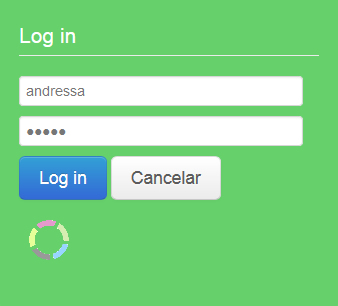
\includegraphics[scale=0.60]{./imagens/login.jpg}}
	\caption[Tela de login ]
	{Tela de login \textbf{Fonte:} Elaborado pelos autores.}
	\label{fig:pagina_login}
\end{figure}

Segundo \citeonline{token_traditional_babal}, os sistemas de autenticações tradicionais utilizam recursos como sessão e \textit{cookies}. A autenticação do usuário é realizada por meio de alguns dados, geralmente nome de usuário (ou email) e senha, com esses dados a aplicação no \textit{back-end}, os validam junto a base de dados e caso obtenha sucesso nesse processo de validação é criada uma sessão e armazenada no servidor, após realizada toda a validação a aplicação retorna a informação dessa sessão para quem a requisitou de modo que ela seja armazenada no navegador de internet por meio de sessão e/ou \textit{cookies}. A partir desse momento, a cada nova solicitação a aplicação \textit{back-end} irá comparar a sessão armazenada no servidor com a fornecida pelo \textit{front-end}. A Fígura~\ref{fig:autenticacao_via_sessao} demonstra o fluxo utilizado pelos sistemas cuja autenticação de sessão é a tradicional.

\newpage
\begin{figure}[h!]
	\centerline{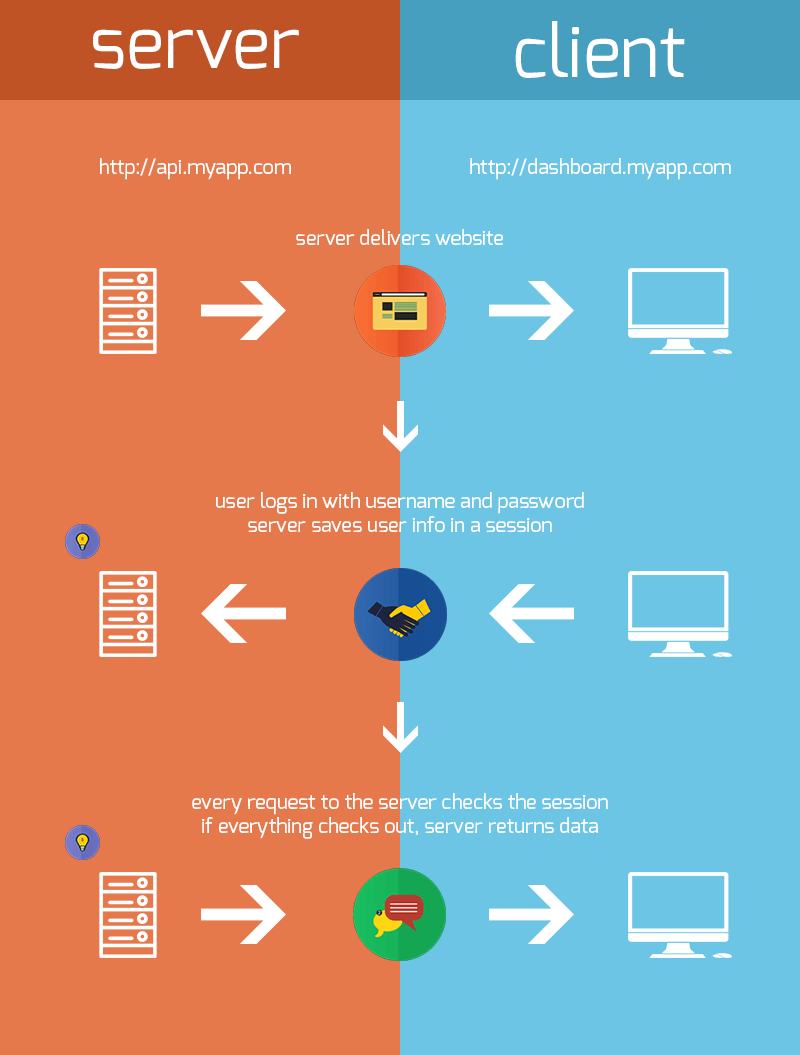
\includegraphics[scale=0.55]{./imagens/tokens-traditional.png}}
	\caption[Fluxo de autenticação de usuários utilizando a forma tradicional]
	{Fluxo de autenticação de usuários utilizando a forma tradicional. \textbf{Fonte:} \cite{authentication_via_token_chris_sevilleja}}
	\label{fig:autenticacao_via_sessao}
\end{figure}

Para \citeonline{authentication_via_token_chris_sevilleja}, a autenticação via \textit{token}, diferente da forma convencional não utiliza os recursos de sessão e \textit{cookies}. Contudo o processo inicial é o mesmo, a autenticação se inicia por meio dos mesmos dados da autenticação tradicional, realiza o mesmo o processo de validação dos dados informados junto a base de dados, porém caso obtenha sucesso não cria uma sessão, e sim um \textit{token} com os dados necessários para a sua validação \textit{criptografados}. Após criado o \textit{token} ele é enviado de volta ao usuário solicitante de modo que ele seja armazenado pela aplicação cliente, sendo ela um aplicativo \textit{web} ou \textit{mobile}, entre outras. A partir desse momento, a cada nova solicitação, a aplicação cliente deverá enviar o \textit{token} anteriormente recebido do servidor e armazenado por ela, para que ele seja validado pelo servidor. A Fígura~\ref{fig:autenticacao_via_token} demonstra o fluxo utilizado pelos sistemas cuja autenticação é realizada via \textit{token}.

\newpage
\begin{figure}[h!]
	\centerline{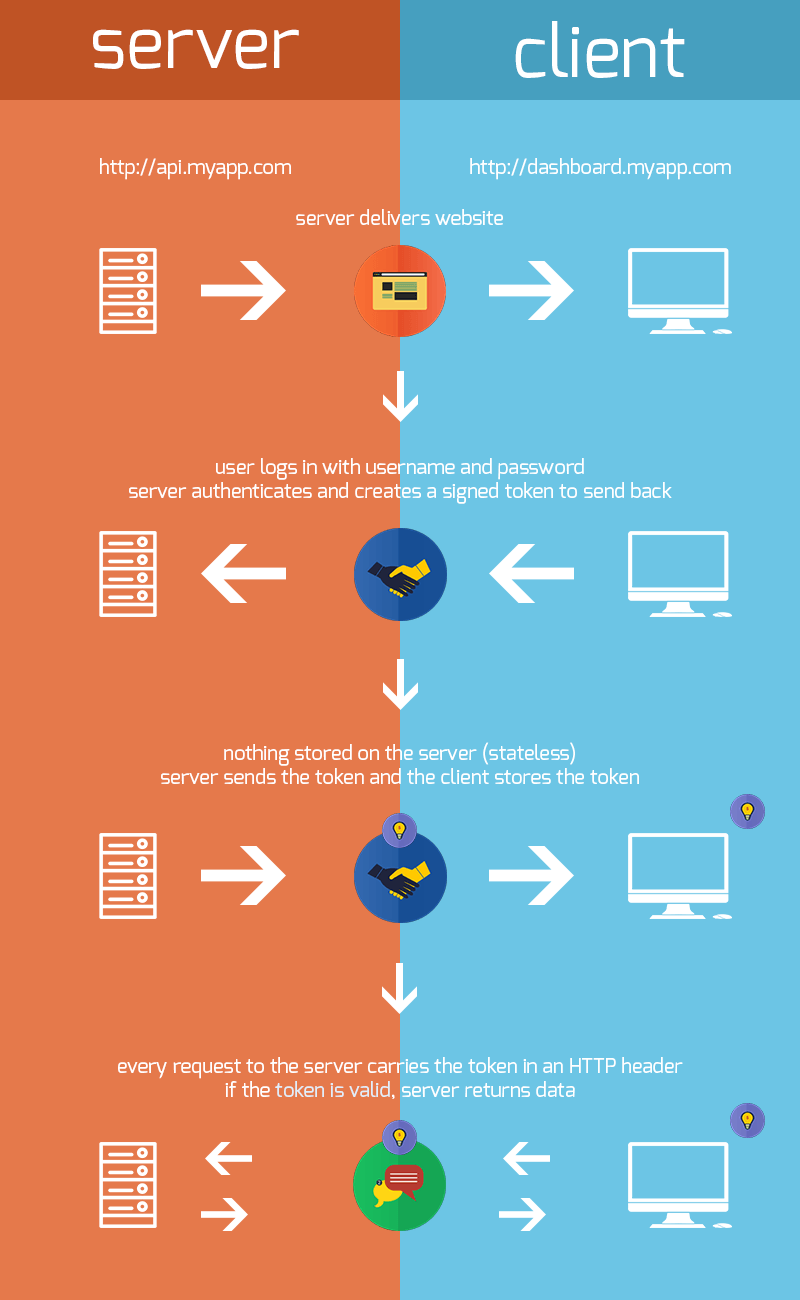
\includegraphics[scale=0.5]{./imagens/tokens-new.png}}
	\caption[Fluxo de autenticação de usuários utilizando \textit{token}]
	{Fluxo de autenticação de usuários utilizando \textit{token}. \textbf{Fonte:} \cite{authentication_via_token_chris_sevilleja}}
	\label{fig:autenticacao_via_token}
\end{figure}

Para construir a aplicação seguindo o modelo de autenticação via \textit{token} foi necessário criar uma classe chamada \texttt{Base64Util} responsável por \textit{criptografar e descriptografar} as informações fornecidas no \textit{token} a fim de validá-lo junto a base de dados da aplicação. Essa classe é apresentada no Código~\ref{list:classe_criptografa_descriptografa_token}.

\begin{lstlisting} [style=custom_Java,caption={[Classe responsável pela criptografia e descriptografia do \textit{token}]{Classe responsável pela criptografia e descriptografia do \textit{token}. \textbf{Fonte:} Elaborado pelos autores.}}, label=list:classe_criptografa_descriptografa_token]
public class Base64Util {
	
	public static final String BASE64_TOKEN_SEPARATOR = "|";
	
	public static byte[] encodeToken(String email, String password) {
		/* Get Current Time in order to check if the session
		 * is valid yet.
		 */
		Long currentTime = new Timestamp(new Date().getTime()).getTime();
		byte[] token = Base64.encode(email + BASE64_TOKEN_SEPARATOR + password + BASE64_TOKEN_SEPARATOR + currentTime);
		return token;
	}
	
	public static Token decodeToken(byte[] tokenDecoded) {
		Token token = new Token();
		
		byte[] bytes = Base64.decode(tokenDecoded);
		String tokenStr = new String(bytes);
		
		String[] splitStr = tokenStr.split("\\" + BASE64_TOKEN_SEPARATOR);
		token.setEmail(splitStr[0]);
		token.setPassword(splitStr[1]);
		token.setLastAccessTime(Long.parseLong(splitStr[2]));
		
		return token;
	}
}
\end{lstlisting}

No código acima, o método chamado \texttt{encodeToken} recebe como parâmetro o \textit{e-mail} e a senha fornecidos pelo usuário no momento da realização do login, a partir dessas informações somado a hora atual do sistema que é obtida na linha 10 é gerado o \textit{token} criptografado em \texttt{Base64}. Para realizar a decodificação do \textit{token} é utilizado o método \texttt{decodeToken} cuja chamada é realizada a cada requisição que o cliente realiza, esse método recebe como parâmentro o \textit{token} criptografado e o descriptografa usando a classe \texttt{Base64} como é apresentado na linha 18. Após a descriptografia dele é criado um objeto da classe \texttt{Token} com as informações obtidas pelo \textit{token} fornecido pela requisição.

Diferentemente das aplicações que utilizam este conceito de sessão via \textit{token}, neste trabalho houve-se a necessidade de validar além das informações do usuário incluídas no próprio \textit{token}, a data e hora da última requisição realizada pelo usuário. Portanto, para validar o \textit{token} expirado foi necessário criar a classe \texttt{TokenBi} como demonstra o Código~\ref{list:classe_valida_token}.

\begin{lstlisting} [style=custom_Java,caption={[Classe responsável pela validação do \textit{token}]{Classe responsável pela validação do \textit{token}. \textbf{Fonte:} Elaborado pelos autores.}}, label=list:classe_valida_token]
public class TokenBi {
	
	private static final int MINUTES_OF_SESSION_ACTIVE = 15; //15min
	...
	
	/* Method to check if session is still alive */
	public boolean isExpiredSession(Token token) {
		
		final long ONE_MINUTE_IN_MILLIS = 60000;//millisecs
		
		Date currentTime = new Date();
		Date timeLastAccess = new Date(token.getLastAccessTime() 
				+ (MINUTES_OF_SESSION_ACTIVE * ONE_MINUTE_IN_MILLIS));
		
		if (timeLastAccess.before(currentTime)) {
			return true; //session already expired
		}
		return false; //session activate yet
	}
	...
}
\end{lstlisting}

Para realizar a validação do \textit{token} expirado, foi criado o método \texttt{isExpiredSession} que  recebe como parâmetro um objeto da classe \texttt{Token} contendo além dos dados do usuário, também a informação relacionada a data e hora da última requisição, com base nessa última informação na linha 12 é realizado um cálculo para obter um objeto do tipo \texttt{Date} contendo a data da última requisição do usuário somado a mais 15 minutos. A partir dessa informação é realizado uma comparação entre ela e a data atual do sistema, como é possível visualizar na linha 15, caso essa informação seja anterior a data atual do sistema o \textit{token} está expirado e o método \texttt{isExpiredSession} retorna \textit{true}. Caso contrário ele irá retornar \textit{false}.

\par Com o funcionamento do sistema de \textit{login}, passou-se a desenvolver a página inicial da aplicação, contendo as informações que são restritas ao usuário cadastrado. O sistema apresenta uma página inicial diferente para cada tipo de conta, sendo elas: contratantes, provedores de serviço ou ambos, contendo apenas as informações que são liberadas de acordo com o acesso do usuário, sendo essas informações relatórios, últimas atualizações na rede de parceiros, avaliações de serviços e prováveis parceiros. A página inicial do tipo contratante é apresentada na Figura~\ref{fig:pagina_inicial_contratante}.

\newpage
\begin{figure}[h!]
	\centerline{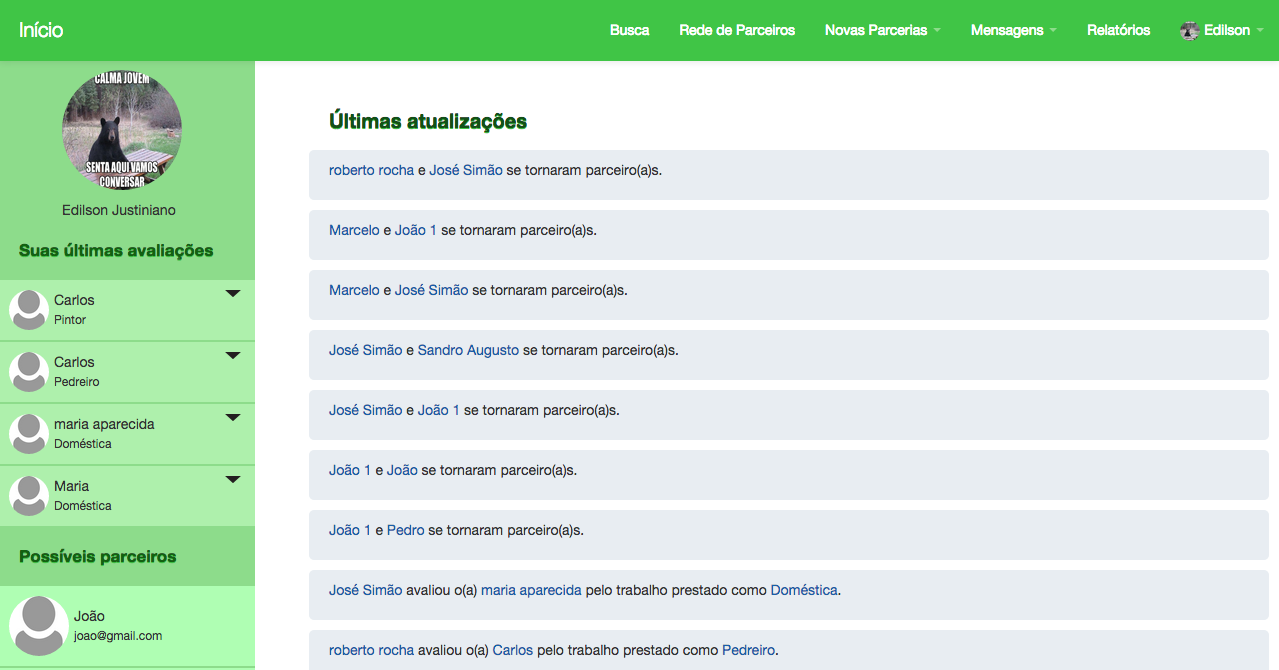
\includegraphics[scale=0.3]{./imagens/home-contratante.png}}
	\caption[Página inicial do usuário contratante]
	{Página inicial do usuário contratante \textbf{Fonte:} Elaborado pelos autores.}
	\label{fig:pagina_inicial_contratante}
\end{figure}


\par O caso de uso localizar parceiros foi desenvolvido após a conclusão do caso de uso criar conta. A lógica deste caso de uso consiste em buscar por possíveis parceiros, com base na rede de parceria do contrante. A Figura~\ref{fig:pagina_localizar_parceiro} apresenta esta busca.

\begin{figure}[h!]
	\centerline{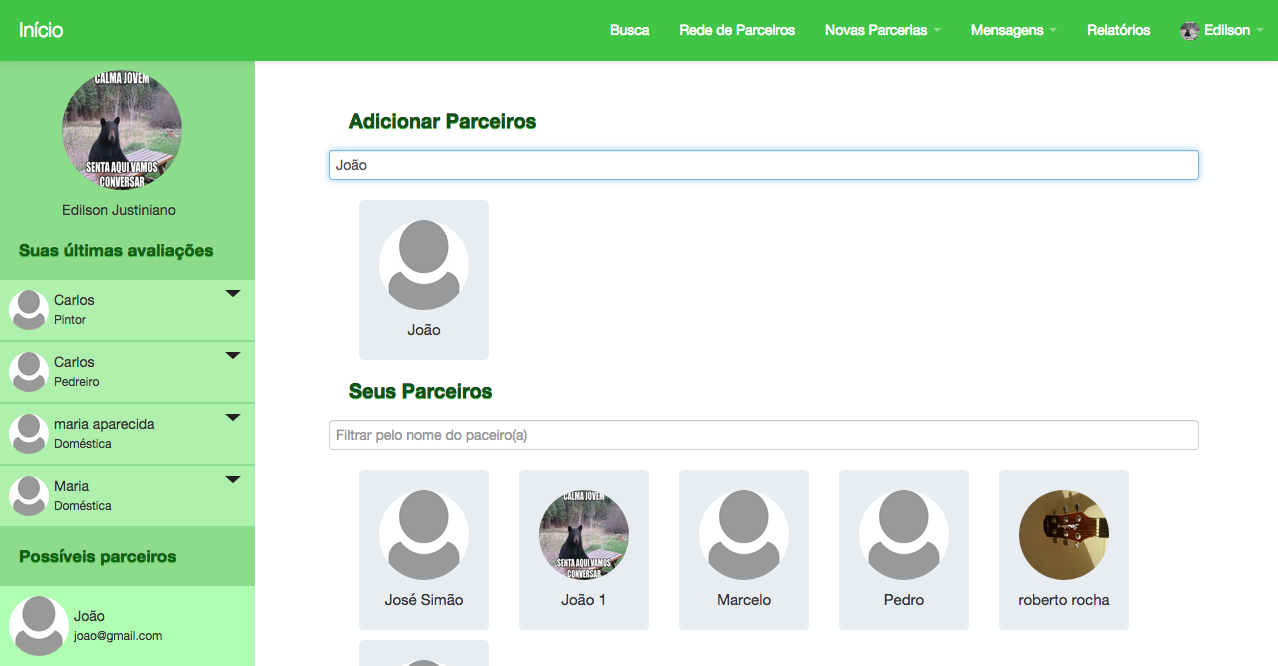
\includegraphics[scale=0.3]{./imagens/localizar-parceiro.png}}
	\caption[Página de localização de parceiros]
	{Página de localização de parceiros \textbf{Fonte:} Elaborado pelos autores.}
	\label{fig:pagina_localizar_parceiro}
\end{figure}

\par Ainda relacionado ao tipo de conta contratante ou ambos, foi implementado o caso de uso adicionar parceiro, que permite ao usuário convidar um possível parceiro para fazer parte da sua rede.

\par Ao enviar a solicitação de parceria, a aplicação executa uma consulta no banco de dados. Essa consulta é responsável por criar uma aresta entre o nó do usuário autenticado no sistema e o parceiro convidado, conforme apresenta o Código~\ref{list:query_adicionar_parceiro}.

\begin{lstlisting} [style=custom_SQL,caption={[\textit{Query} para enviar solicitação de parceria]{\textit{Query} para enviar solicitação de parceria. \textbf{Fonte:} Elaborado pelos autores.}}, label=list:query_adicionar_parceiro] 	
MATCH (me:Person {email: 'edilsonjustiniano@gmail.com'}),
(partner:Person {email: 'andressa_faria18@hotmail.com'})
CREATE (me)-[:PARTNER_OF {since: 9898723435424281}]->(partner)
RETURN {myName: me.name, myEmail: me.email, partnerName: partner.name, 
partnerEmail: partner.email} as added
\end{lstlisting}

\par Essa consulta é separada em três partes, sendo elas dividas pelas cláusulas \texttt{MATCH}, \texttt{CREATE} e \texttt{RETURN}. A primeira parte dessa consulta irá localizar os vértices cujos \textit{e-mails} sejam semelhantes ao do usuário autenticado no sistema e do parceiro convidado, respectivamente. A segunda parte é responsável por criar a aresta entre os vértices obtidos pela primeira parte da consulta. A terceira e última parte, irá retornar os dados de ambos os usuários, sendo eles, o usuário autenticado no sistema e parceiro recém convidado a fazer parte da rede de parceiros do usuário autenticado.

\par Após a implementação da lógica para adicionar um novo parceiro, houve a necessidade de implementar o serviço de requisições de parcerias, uma vez que não bastava apenas um contratante convidar outro para se tornarem parceiros, mas sim que o contratante convidado aceitasse sua solicitação de parceria, para assim se tornarem parceiros. Visando disponibilizar estas solicitações de forma agradável ao usuário, foi desenvolvida uma funcionalidade para que o usuário pudesse aceitar ou rejeitar a solicitação enviada à ele, essa funcionalidade apresentada em destaque na Figura~\ref{fig:aceitar_rejeitar_solicitacao_parceria}.

\begin{figure}[h!]
	\centerline{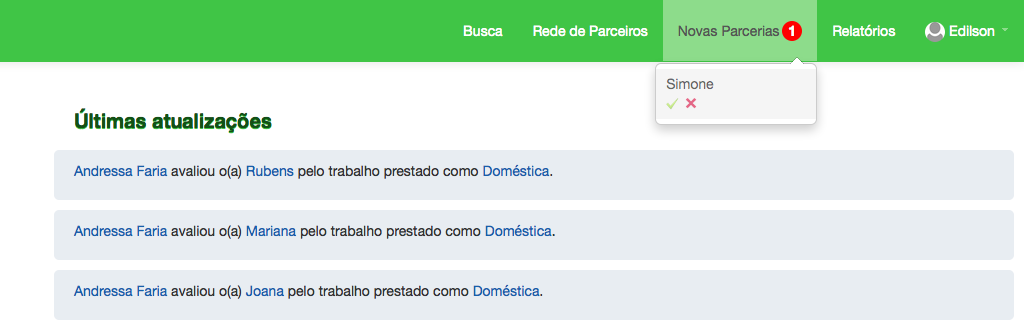
\includegraphics[scale=0.45]{./imagens/aceitar_rejeitar_solicitacao_parceria.png}}
	\caption[Tela para aceitar ou rejeitar solicitação de parceria]
	{Tela para aceitar ou rejeitar solicitação de parceria. \textbf{Fonte:} Elaborado pelos autores.}
	\label{fig:aceitar_rejeitar_solicitacao_parceria}
\end{figure}

\par A partir dessa funcionalidade, o usuário será capaz de aceitar ou recusar a solicitação apenas com um \textit{click}. Caso o usuário aceite a solicitação, o sistema irá realizar os procedimentos necessários e irá executar a mesma consulta apresentada no Código~\ref{list:query_adicionar_parceiro}, porém com os \textit{e-mails} invertidos. Essa consulta será reutilizada, pois, para que dois usuários se tornem parceiros é necessário que ambos possuam uma aresta do tipo \texttt{PARTNER OF} apontando um ao outro.

\par Se o usuário rejeitar a solicitação, o sistema realizará os procedimentos necessários e executará a consulta apresentada no Código~\ref{list:query_remover_parceiro} a fim de excluir a aresta criada anteriormente pela solicitação de parceria.

\begin{lstlisting} [style=custom_SQL,caption={[\textit{Query} para remover solicitação de parceria]{\textit{Query} para remover solicitação de parceria. \textbf{Fonte:} Elaborado pelos autores.}}, label=list:query_remover_parceiro] 	
MATCH (me:Person {email: 'andressa_faria18@hotmail.com'}),
(partner:Person {email: 'edilsonjustiniano@gmail.com'}),
(partner)-[rel:PARTNER_OF]->(me)
DELETE rel
RETURN {myName: me.name, myEmail: me.email, 
partnerName: partner.name, partnerEmail: partner.email} as deleted;
\end{lstlisting}

\par Essa consulta, a exemplo da anterior, é separada em três partes, sendo elas dividas pelas cláusulas \texttt{MATCH}, \texttt{DELETE} e \texttt{RETURN}. A primeira parte dessa consulta irá localizar os vértices cujos \textit{e-mails} sejam semelhantes ao do usuário autenticado no sistema e do parceiro convidado, respectivamente, e que possuam uma aresta do tipo \texttt{PARTNER OF} os conectando, porém, essa aresta se inicia no vértice relacionado ao parceiro convidado e o final seja vértice relacionado ao usuário autenticado. A segunda parte consiste apenas na exclusão da aresta obtida na primeira parte da consulta. A terceira e última parte, irá retornar os dados de ambos os usuários, sendo eles, o usuário autenticado no sistema e parceiro cujo, convite para se tornar parceiro foi rejeitado pelo usuário autenticado no sistema.

\par Após realizada a implementação do caso de uso adicionar parceiro, houve a necessidade de desenvolver a busca por todos os usuários que possuíam o tipo de conta contratante ou ambos e que possuíam um relacionamento de parceria com o usuário autenticado no sistema, além da funcionalidade de localizar novos parceiros, baseando-se na localização da empresa na qual o usuário trabalha e na cidade onde ele vive, sempre ordenando os resultados por meio da quantidade de parceiros em comum. 

\par O caso de uso gerenciar serviços foi implementado em sequência, abrangendo as principais funcionalidades de gerenciamento: cadastrar e adicionar um novo serviço ao usuário, cujo tipo de conta é provedor de serviços, listar os serviços atribuídos a ele, e remover serviços quando necessário. Visando melhorar a usabilidade, foi implementado um mecanismo de busca, que permitiu filtrar os resultados por meio de um campo que possui a função  auto completar, evitando assim, possíveis erros e diminuindo o tempo gasto pelo usuário para adicionar o serviço. A função realiza a busca em uma lista de serviços anteriormente cadastrados, no entanto, caso não haja o serviço solicitado, o usuário tem a liberdade de cadastrá-lo e atribuí-lo a si mesmo.

\par A partir deste ponto, foi possível iniciar o desenvolvimento do caso de uso "localizar mão de obra", uma vez que, este caso de uso dependia diretamente das implementações das funcionalidades adicionar parceiros para os usuários contratantes e adicionar serviços aos provedores de serviço. Para facilitar a localização e deixar o \textit{software} mais usual, esta busca se baseia inicialmente no serviço buscado pelo usuário, sendo posteriormente modificada para também levar em consideração a funcionalidade avaliar serviço que foi implementada paralelamente. A avaliação de serviço permite ao contratante dar uma nota ao serviço que foi prestado a ele. Com estas informações foi possível desenvolver uma busca que levaria em consideração, além destas informações, a rede de parceiros do usuário contratante, a fim de lhe apresentar as melhores opções possíveis.

\par A fim de abranger a busca e possibilitar que novos prestadores de serviços sejam avaliados pelos contratantes, a consulta que antes apresentava apenas provedores de serviços que possuíam avaliações, sendo elas, positivas ou negativas, foi ampliada, possibilitando que profissionais não avaliados também entrassem na lista de prováveis provedores de serviços.

\par Para auxiliar na tomada de decisão do usuário contratante, foi implementada uma funcionalidade que realiza o cálculo da média de avaliações de um serviço prestado por um profissional temporário, tendo como base as avaliações já realizadas pela rede de parceiros do usuário autenticado, da empresa onde ele trabalha e da cidade onde vive, oferecendo assim uma forma simples de obter acesso a qualidade do serviço prestado.

\par Após realizada todas as implementações já descritas, houve a preocupação de desenvolver uma interface, que além de amigável fosse prática ao usuário, desta forma, foi disponibilizada algumas informações relevantes, que auxiliam o usuário a compreender o que está ocorrendo em sua rede de parceria. Como exemplo é possível citar a lista de parceiros em comum entre o usuário autenticado no sistema e um determinado contratante por meio da página de perfil dele.

\par A fim de agregar mais funcionalidades para o usuário provedor de serviços, foi criado na página inicial do \textit{software} uma funcionalidade que visa apresentar algumas dicas interessantes que contribui com a sua imagem perante ao \textit{software}, levando-o assim a obter uma quantidade maior de oportunidades de trabalho.

\par Para finalizar o desenvolvimento será necessário desenvolver alguns gráficos que apresentem ao usuário informações a respeito da qualidade do serviço prestado pelo provedor de serviços, comparando-os com os demais prestadores, porém estes gráficos ainda não foram implementados até o momento.
